\section{Workload analysis}
\label{sec:dataset-analysis}

%\subsection{Layer size distribution}
%
%\subsection{File size distribution}
%
%\subsection{Redundant file distribution}

%\section{Deduplication performance analysis} % just find the problem and benefit
\label{sec:background}

%\paragraph{Deduplication for improving storage capacity.}

On-cloud global deduplication software is widely adopted by cloud enterprises for reducing cloud storage consumption and overall storage cost. 
For example, StorReduce~\cite{storReduce}, the deduplication software used by
Google cloud and AWS, 
performs in-line transparent data deduplication. 
%StorReduce resides between the client's application and the hosting cloud storage.
%A number of deduplication methods focus on client-side data deduplication to ensure that only unique files are uploaded, 
%to save network bandwidth, by having the client send a duplicate check request~\cite{xxx}~\cite{xxx}. 
%For example, xxxx\NZ{Hadeel, can you add one example and few relatedwork citation?}. 
Intuitively, such deduplication techniques can be leveraged to eliminate redundant data from the Docker image storage system.  
Except, the Docker image dataset is not amenable to deduplication 
as the images are \emph{compressed archival files}.
%Intuitively, registries can be deployed as a proxy cache to host frequently requested layers to speedup image pulls and improve performance 
%while the backend cloud storage can leverage deduplication to save storage space.
%However, there are several unique problems concerning the integration of caching and deduplication to the unique Docker registries workload: \textbf{compressed layers}. 
%We investigate the potential for data reduction in the Docker registry by estimating the efficacy of layer sharing and file-level deduplication.
%We noticed that the number of public repositories is constantly increasing with a growth that amounts 
%to around 1 million repositories annually. 
%This corresponds to~130\,TB of annual growth in storage needs 
%\HA{but it is actually less because of shared layers, right?}, 
%costing around~\$15,000 a month if Google Cloud Storage is used~\cite{GoogleCloudStoragePricing}.
%This growth implies significant benefits to data deduplication. 


As discussed in~\cref{sec:intro}, only $3$\% of the files in a sample Docker hub image collection were found to be unique, mainly becuase 
 compressed files have a very low deduplication ratio~\cite{meister2012study}.
Thus, 
we can realize significant space savings if we can remove the 
duplicate files. This entails decompressing files before performing deduplication, and collecting components of layers from multiple servers.
%
To quantify the performance overhead of such an approach involving decompressing, deduplication, and then re-compressing,
we setup five registry instances. Each instance has a local file system as their backend storage system. We
implemented file-level deduplication with decompression and compression operations.
We replayed the IBM registry workload \texttt{dal}~\cite{dockerworkload} 
%by sending requests randomly 
randomly to our five registries and measured the latency. 
%
Figure~\ref{fig:avg_latency_dedup_nodedup} shows the average latency observed 
across five registries.
%\arb{average across what??}\NZ{addressed}.
Note that since 
%the IBM registry workload 
\texttt{dal} does not contain real layers,
we extract the layer digest from each request and match it with a layer randomly selected from our Docker Hub dataset to emulate realistic requests.

Without deduplication,
the average latency for requesting a layer is about $2$~s for layers with sizes $\textless50$~MB.
The latency increases to $12$~s when the above deduplication is implemented in the backend storage system.
Furthermore, Docker registry performance drops down dramatically for larger layers.
We observe that the average latency for requesting layers $\textgreater50$~MB and $\textless1$~GB
is about $128$~s. The latency worsens with dedupliation to on average of about $800$~s.
%\NZ{todo:graph: less than, }
%\HA{running five registries, replaying dal trace using trace replayer-cite, and since the replayer doesn't use real layers we randomly match the request to our dataset downloaded from docker hub. describe how we got these numbers. for dedup, we simply implemented a decompress/compress + file-level deduplication on backend storage systems, we use a CHT based distributed storage system. Figure~\ref{fig:avg_latency_dedup_nodedup}}
\begin{figure}[t]
	\centering
	%\scriptsize
	\begin{minipage}{0.225\textwidth}
		\centering
		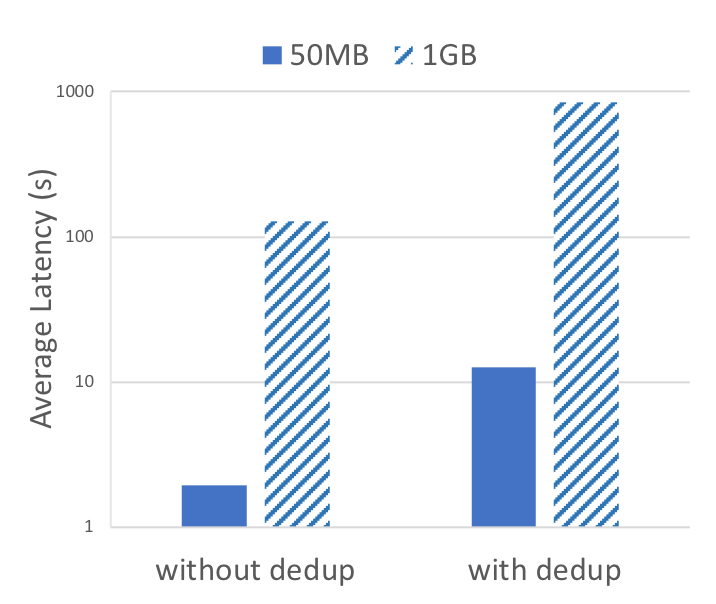
\includegraphics[width=1\textwidth]{graphs/avglatency_dedup_nodedup.png}
		\caption{Average latency.}
		\label{fig:avg_latency_dedup_nodedup}
	\end{minipage}
	\begin{minipage}{0.225\textwidth}
		\centering
		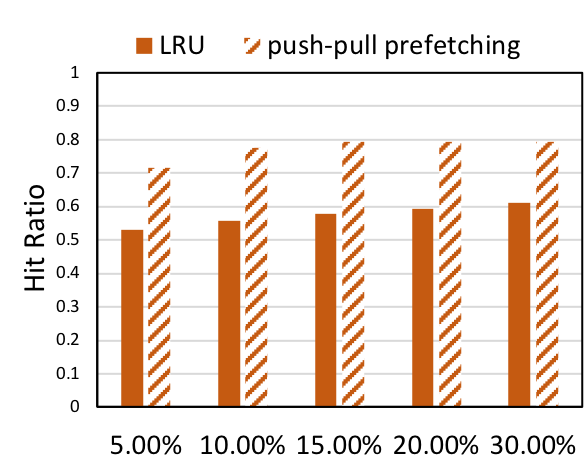
\includegraphics[width=1\textwidth]{graphs/lru_prefetch_hits.png}
		\caption{Hit ratio.}
		\vspace{-3pt}
		\label{fig:lru_prefetching_hits}
	\end{minipage}
\end{figure}
% for LRU and push-pull prefetching under different cache sizes (\% of total accessed layers).


Before describing Sift, we must understand the trends in the access patterns of the Docker registries at the layer and repository level. INSERT DESCRIPTION OF DATASET HERE.
%\subsubsection{User access pattern based preconstruction}
%
%Docker client stores images as lists of layers and layers are shared among different repositories, 
%which is similar to Docker registry.
%When a client pulls an image from a repository, 
%it will first \texttt{pull} the manifest of the image~\cite{docker}~\cite{dockerworkload} and 
%parse the manifest to get the layer digests,
%then lookup each layer digest against a \emph{local layer index}.
%After that it only pulls the layers that have \emph{not been stored locally}.
%Theoretically, clients only pull layer once. 
%However, some clients may delete several local images and \emph{repull} layers for these images.
%%Moreover, kubernetes allows users always \emph{repull} layers no matter these layers locally available or not~\cite{docker}.  
%Here, a \emph{repull layer} indicates a layer a user pulls multiple times,
%and a \emph{non-repull layer} means users only pull this layer once.
%
%\preconstructcachename~starts parallel slice restoring for layers 
%when a \texttt{pull manifest} request is received, 
%which is called layer preconstruction.
%These preconstructed layer slices are temporally stored in the cache for later \texttt{pull slice} requests.
%In this case, slice restoring process and its overhead can be avoided if the requested slice is found in the cache.
%Next, we analyze user access patterns to identify which layers in the repository will be pulled by users after 
%\texttt{pull manifest} requests.

\subsection{User access patterns}
%\begin{figure*}[t]
%		\begin{minipage}{0.32\linewidth}
%			\centering
%			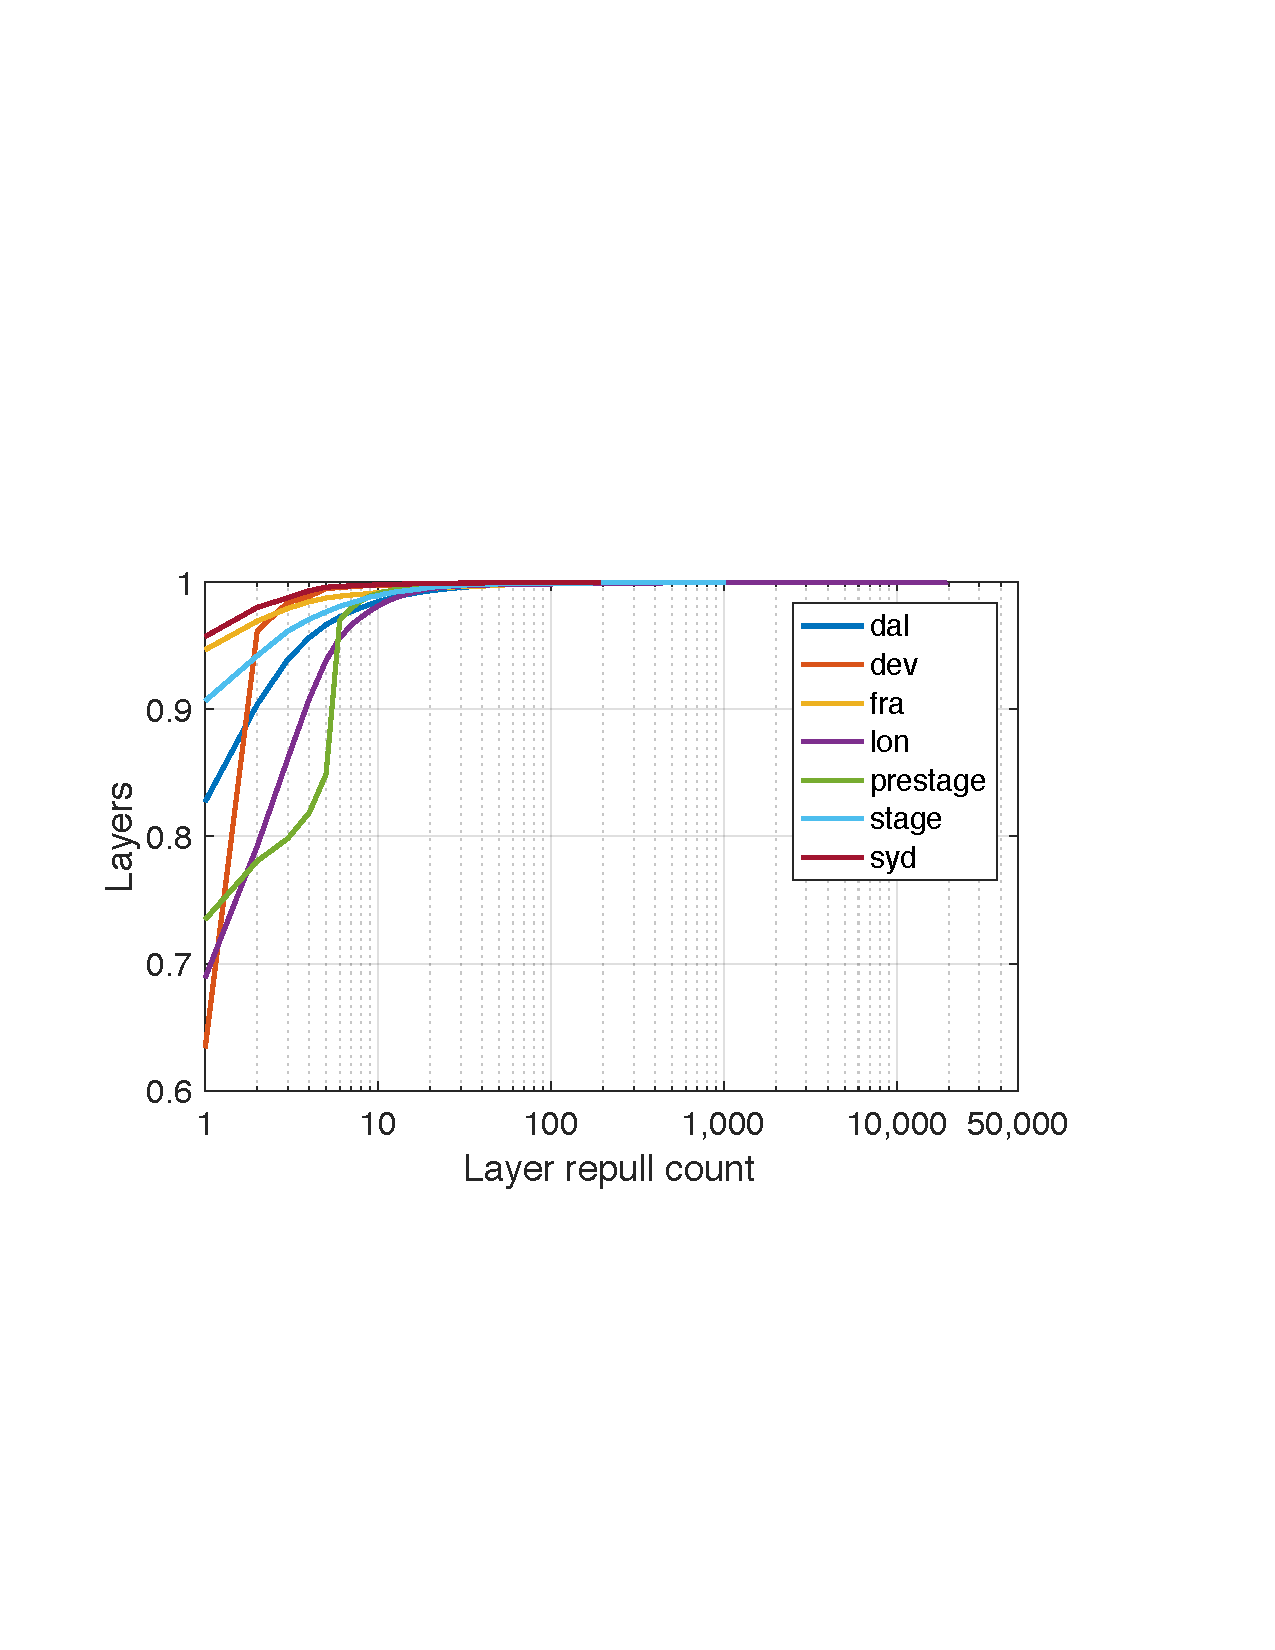
\includegraphics[width=1\textwidth]{graphs/cdf-layer-repull-by-same-client.pdf}
%			%\caption{CDF of layer repull count.}
%		%	\vspace{-3pt}
%			\label{fig:layer-repull-cdf}
%		\end{minipage}
%			\begin{minipage}{0.32\linewidth}
%				\centering
%				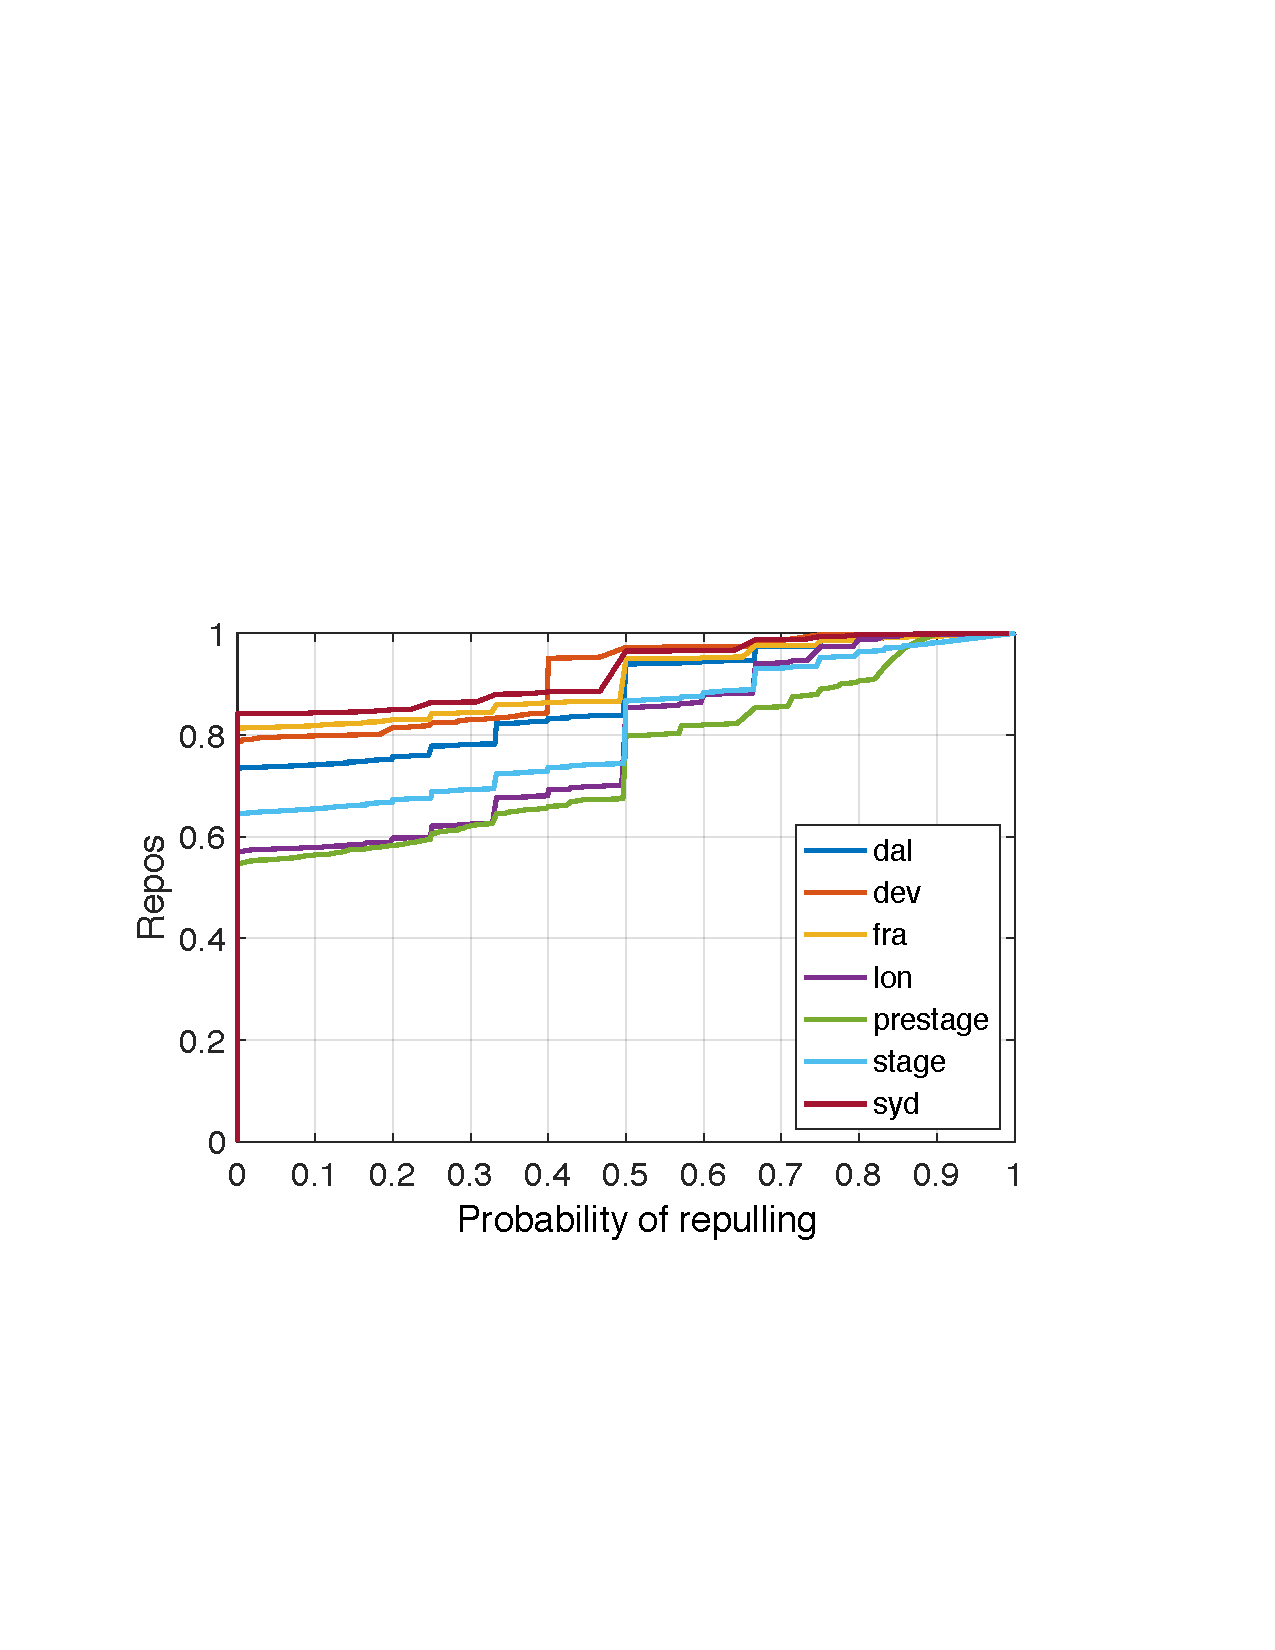
\includegraphics[width=1\textwidth]{graphs/cdf-repo-repull-ratio-by-same-client.pdf}
%				%\caption{PDF of repository repulling probability.}
%				%	\vspace{-3pt}
%				\label{fig:repo-repull-cdf}
%			\end{minipage}
%		\begin{minipage}{0.32\linewidth}
%			\centering
%			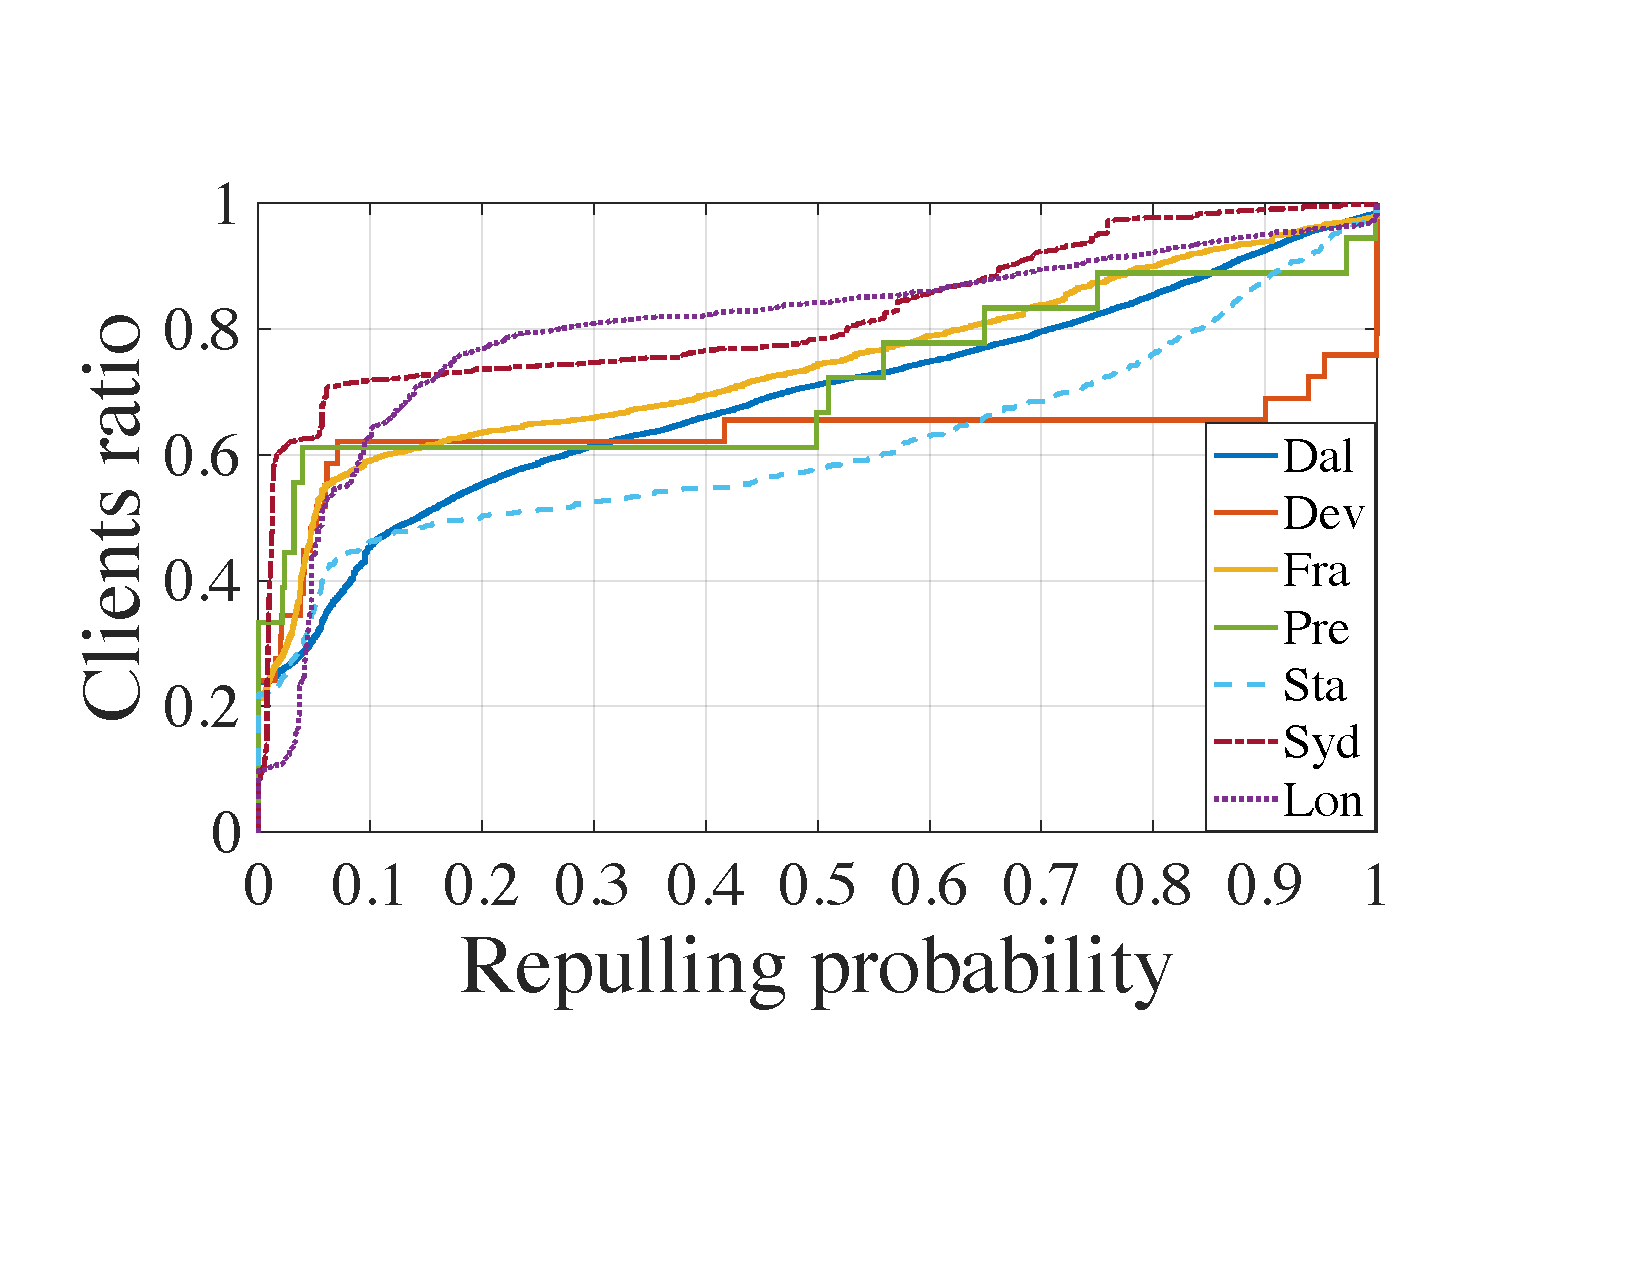
\includegraphics[width=1\textwidth]{graphs/cdf-client-repull-layer-request-ratio.pdf}
%			%
%			%	\vspace{-3pt}
%			\label{fig:client-repull-cdf}
%		\end{minipage}
%	\caption{PDF of client repull count, repository repulling probability, and client repulling probability..}
%\end{figure*}

%\begin{figure}[!t]
%	\centering
%	\subfigure[\texttt{GET} layer request count]{
%		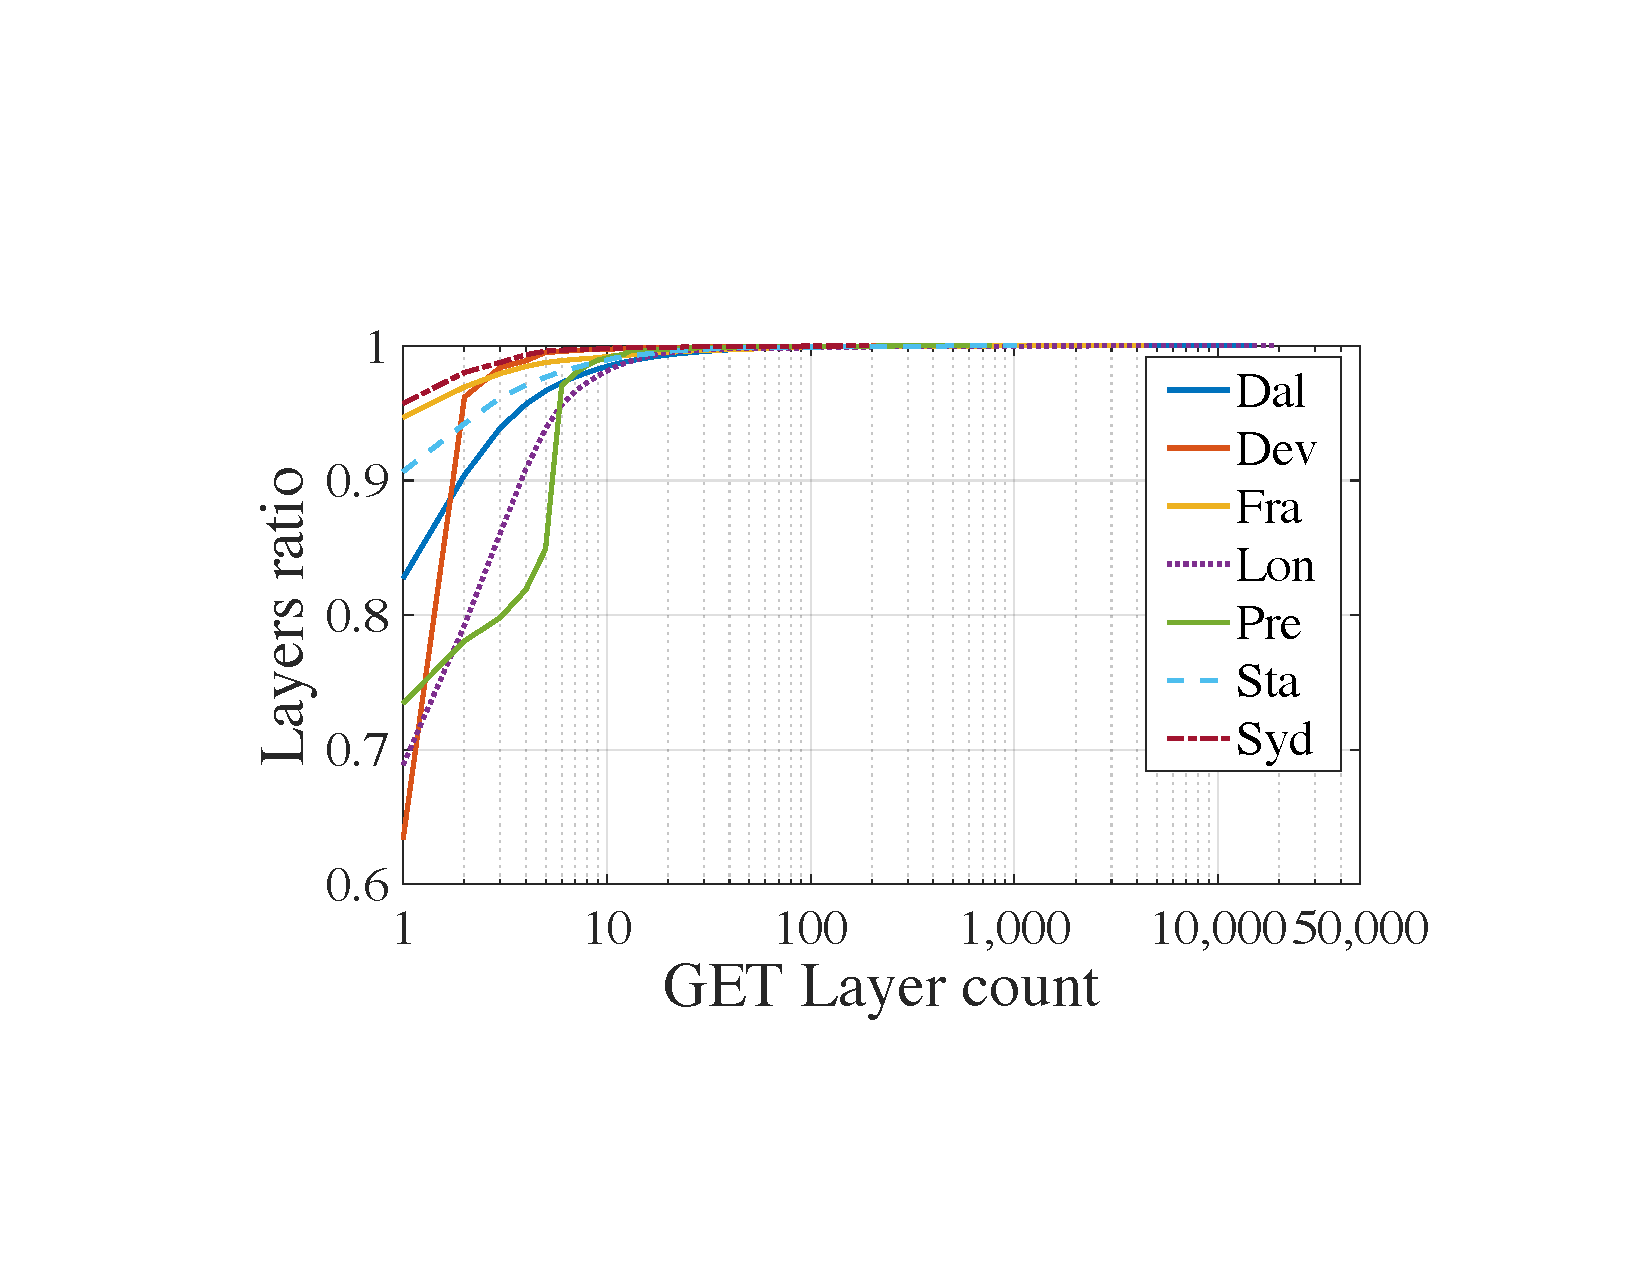
\includegraphics[width=0.22\textwidth]{graphs/cdf-layer-repull-ratio-by-same-client.pdf}
%		\label{fig:layer-repull-cdf}
%	}
%%	\subfigure[Repository repulling probability]{
%%		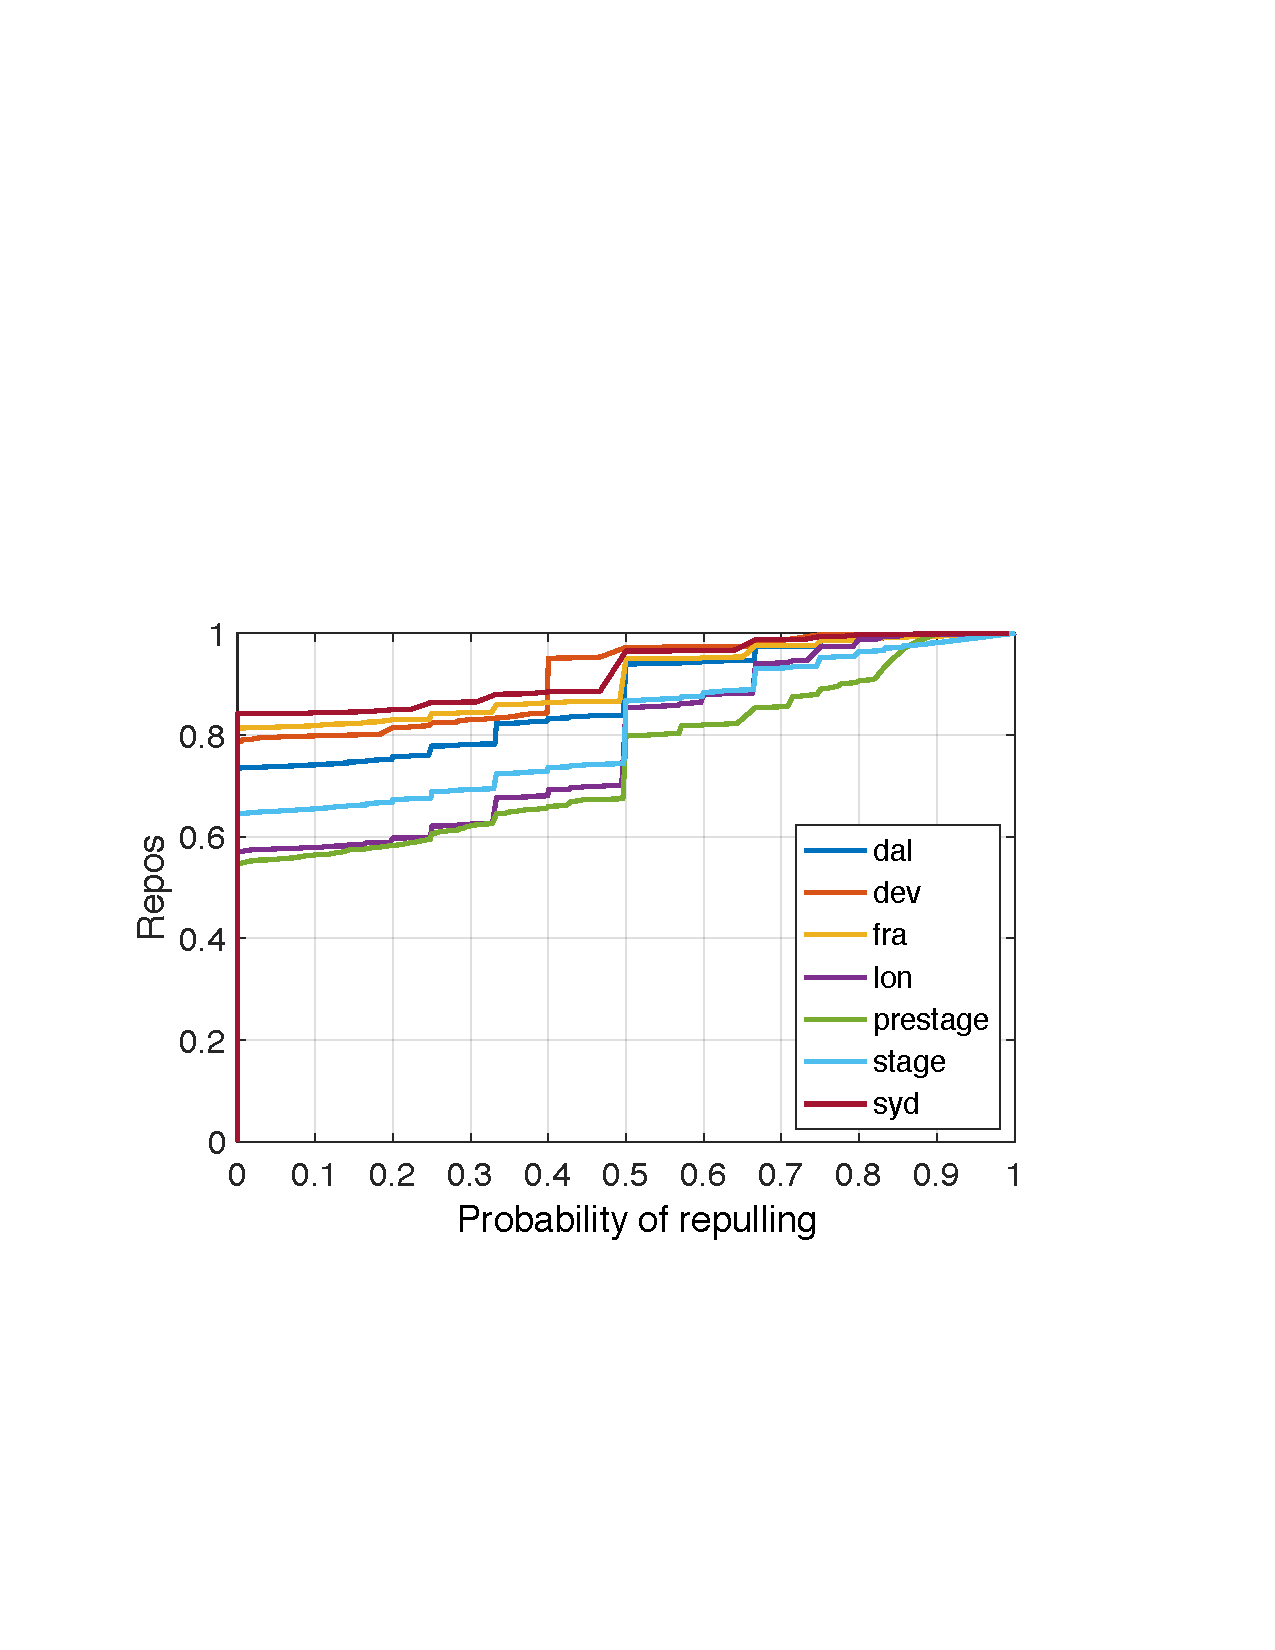
\includegraphics[width=0.2\linewidth]{graphs/cdf-repo-repull-ratio-by-same-client.pdf}
%%		\label{fig:repo-repull-cdf}
%%	}
%	\subfigure[Client repulling probability]{
%	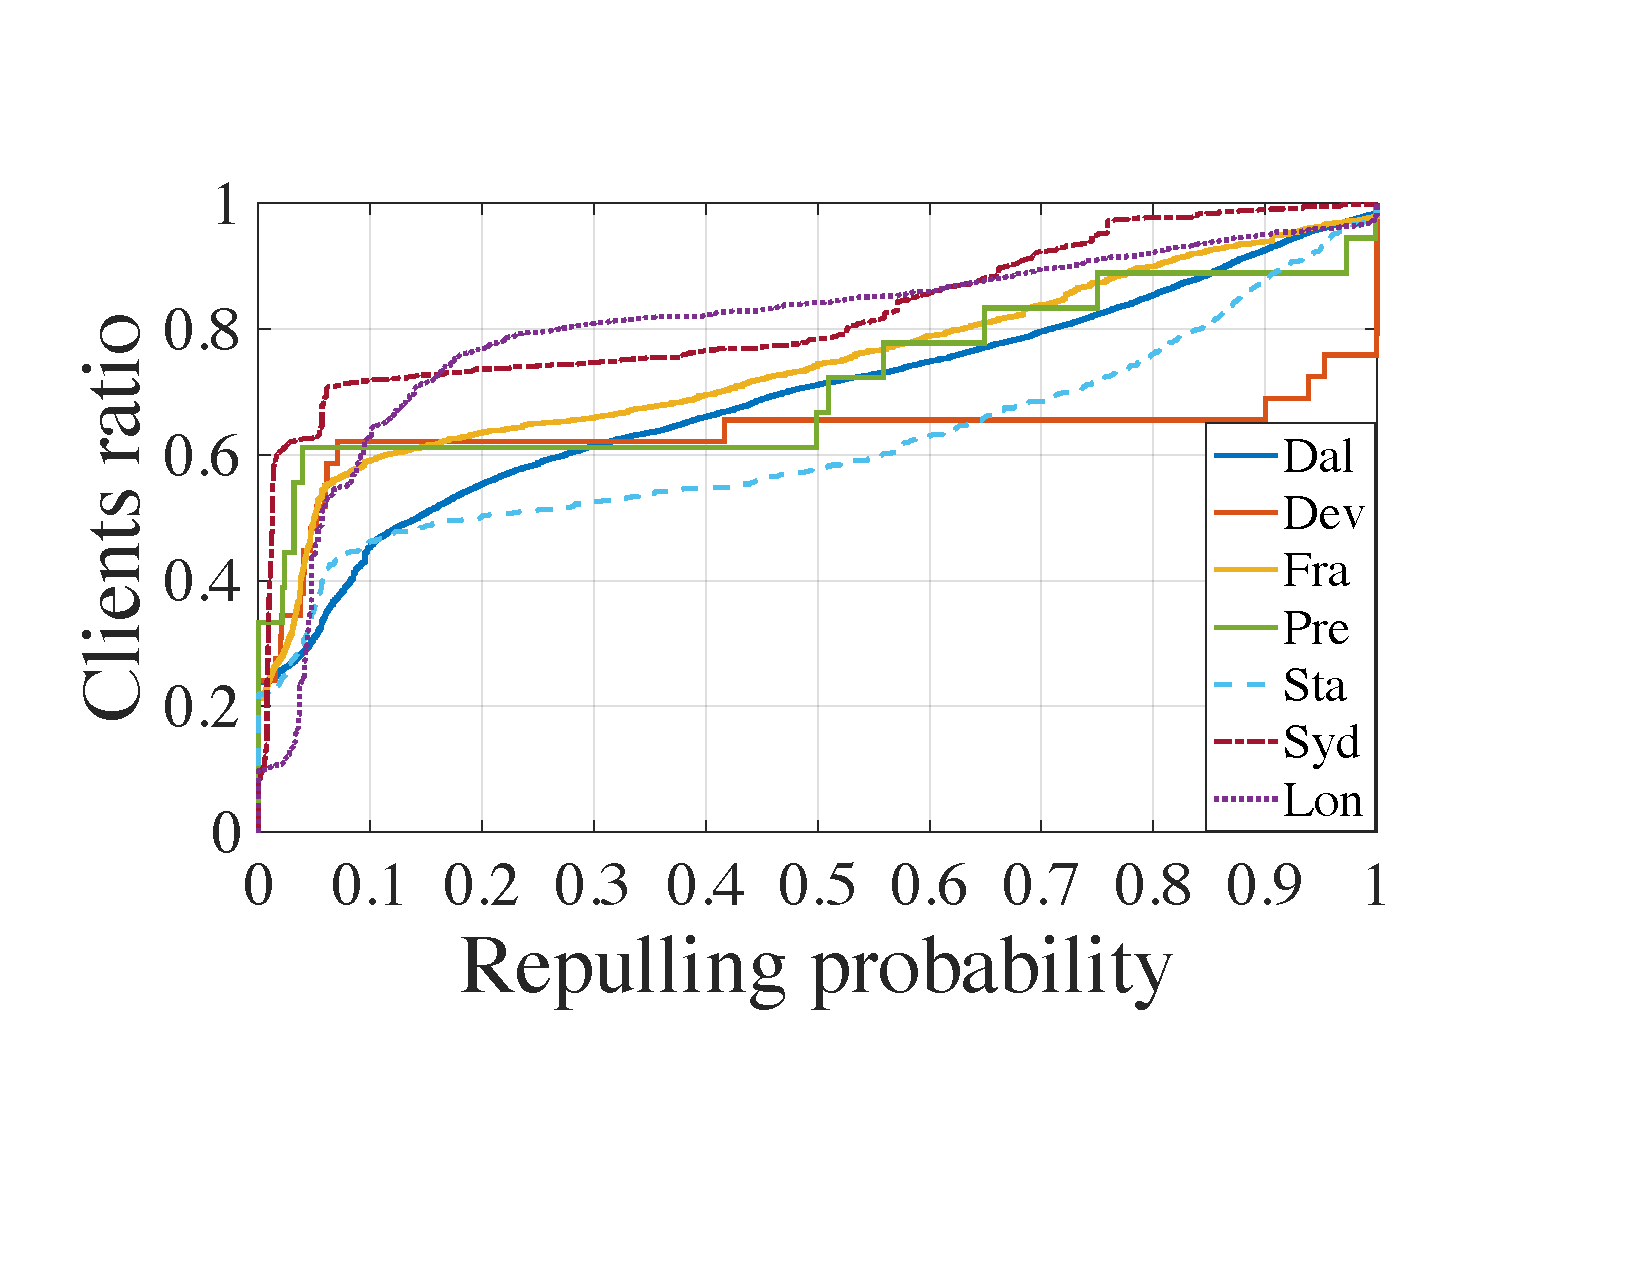
\includegraphics[width=0.2\textwidth]{graphs/cdf-client-repull-layer-request-ratio.pdf}
%   \label{fig:client-repull-cdf}
%}
%	\caption{CDF of \texttt{GET} layer request count and client repulling probability.}
%	\label{fig-repull}
%\end{figure}
%






\begin{figure*}[t]
        \centering
        \begin{minipage}{0.3\textwidth}
                \centering
                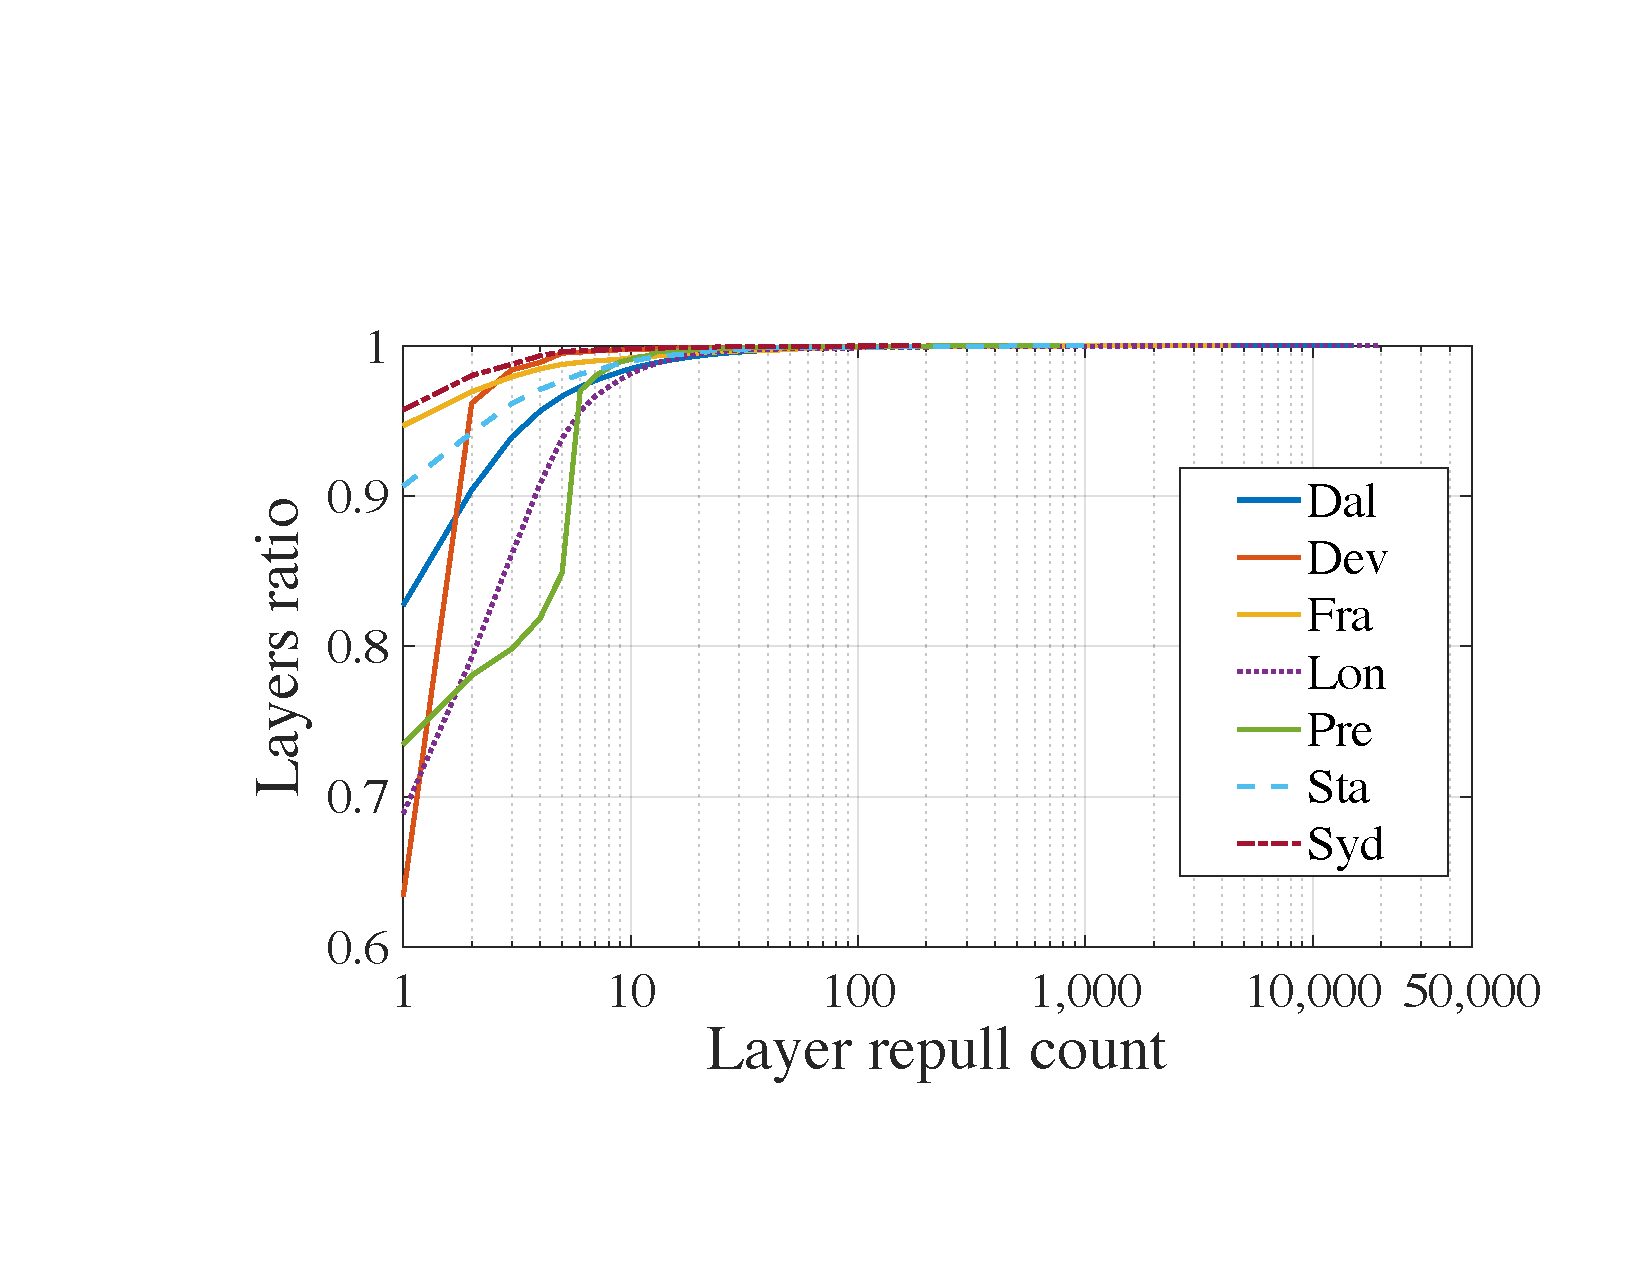
\includegraphics[width=0.9\textwidth]{{graphs/cdf-layer-repull-ratio-by-same-client.pdf}
                \caption{CDF of \texttt{GET} layer request count}
                \label{fig:layer-repull-cdf}
        \end{minipage}%
        \begin{minipage}{0.3\textwidth}
                \centering
                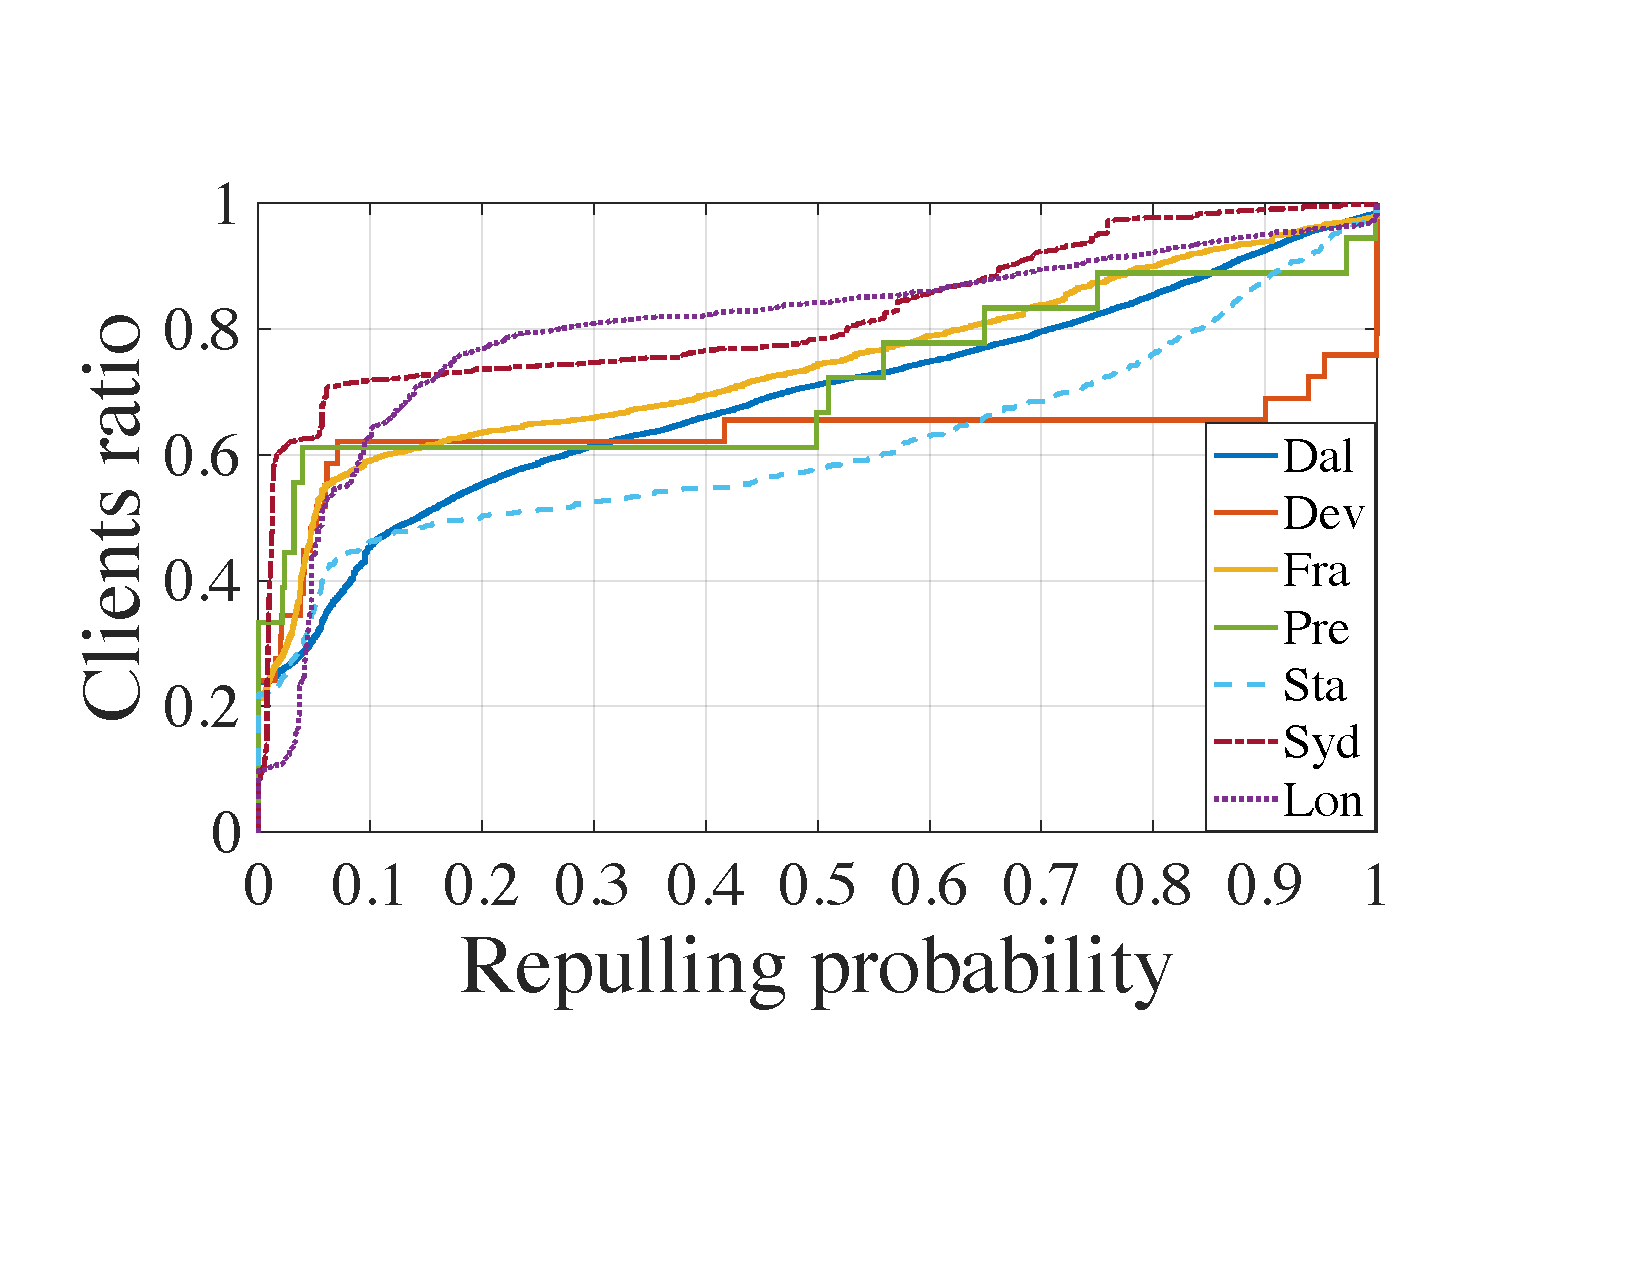
\includegraphics[width=0.9\textwidth]{graphs/cdf-client-repull-layer-request-ratio.pdf}
                \caption{CDF of Client repulling probability}% of LRU cache and preconstruct cache.}
                \label{fig:client-repull-cdf}
        \end{minipage}%
        \begin{minipage}{0.3\textwidth}
        \centering
        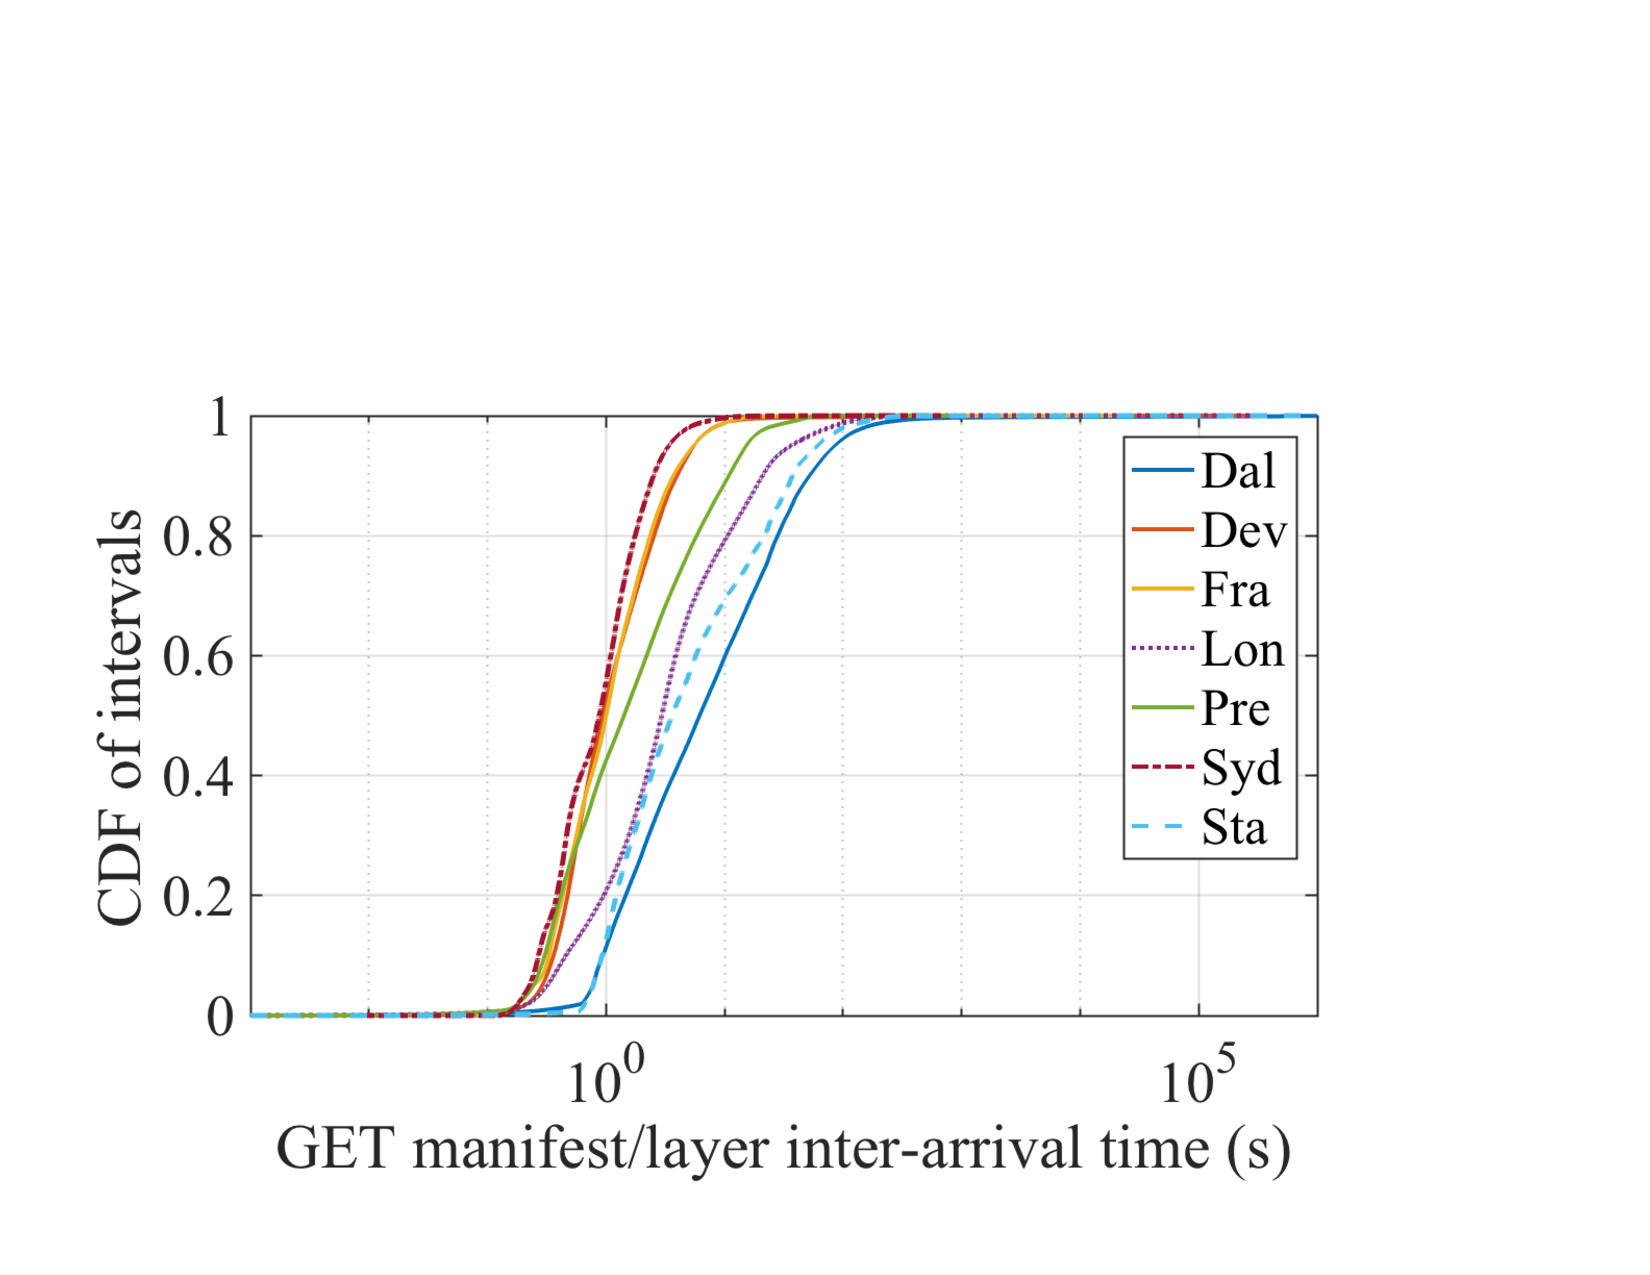
\includegraphics[width=0.9\textwidth]{graphs/GML-intervals.pdf}
        \caption{Intervals between \texttt{GET} manifest request and \texttt{GET} layer request}
        \label{fig:intervals}
   \end{minipage}
\end{figure*}





%\begin{figure}[!t]
%	\centering
%	\subfigure[CDF of compression ratio]{\label{fig_cdf_compression_ratio}
%		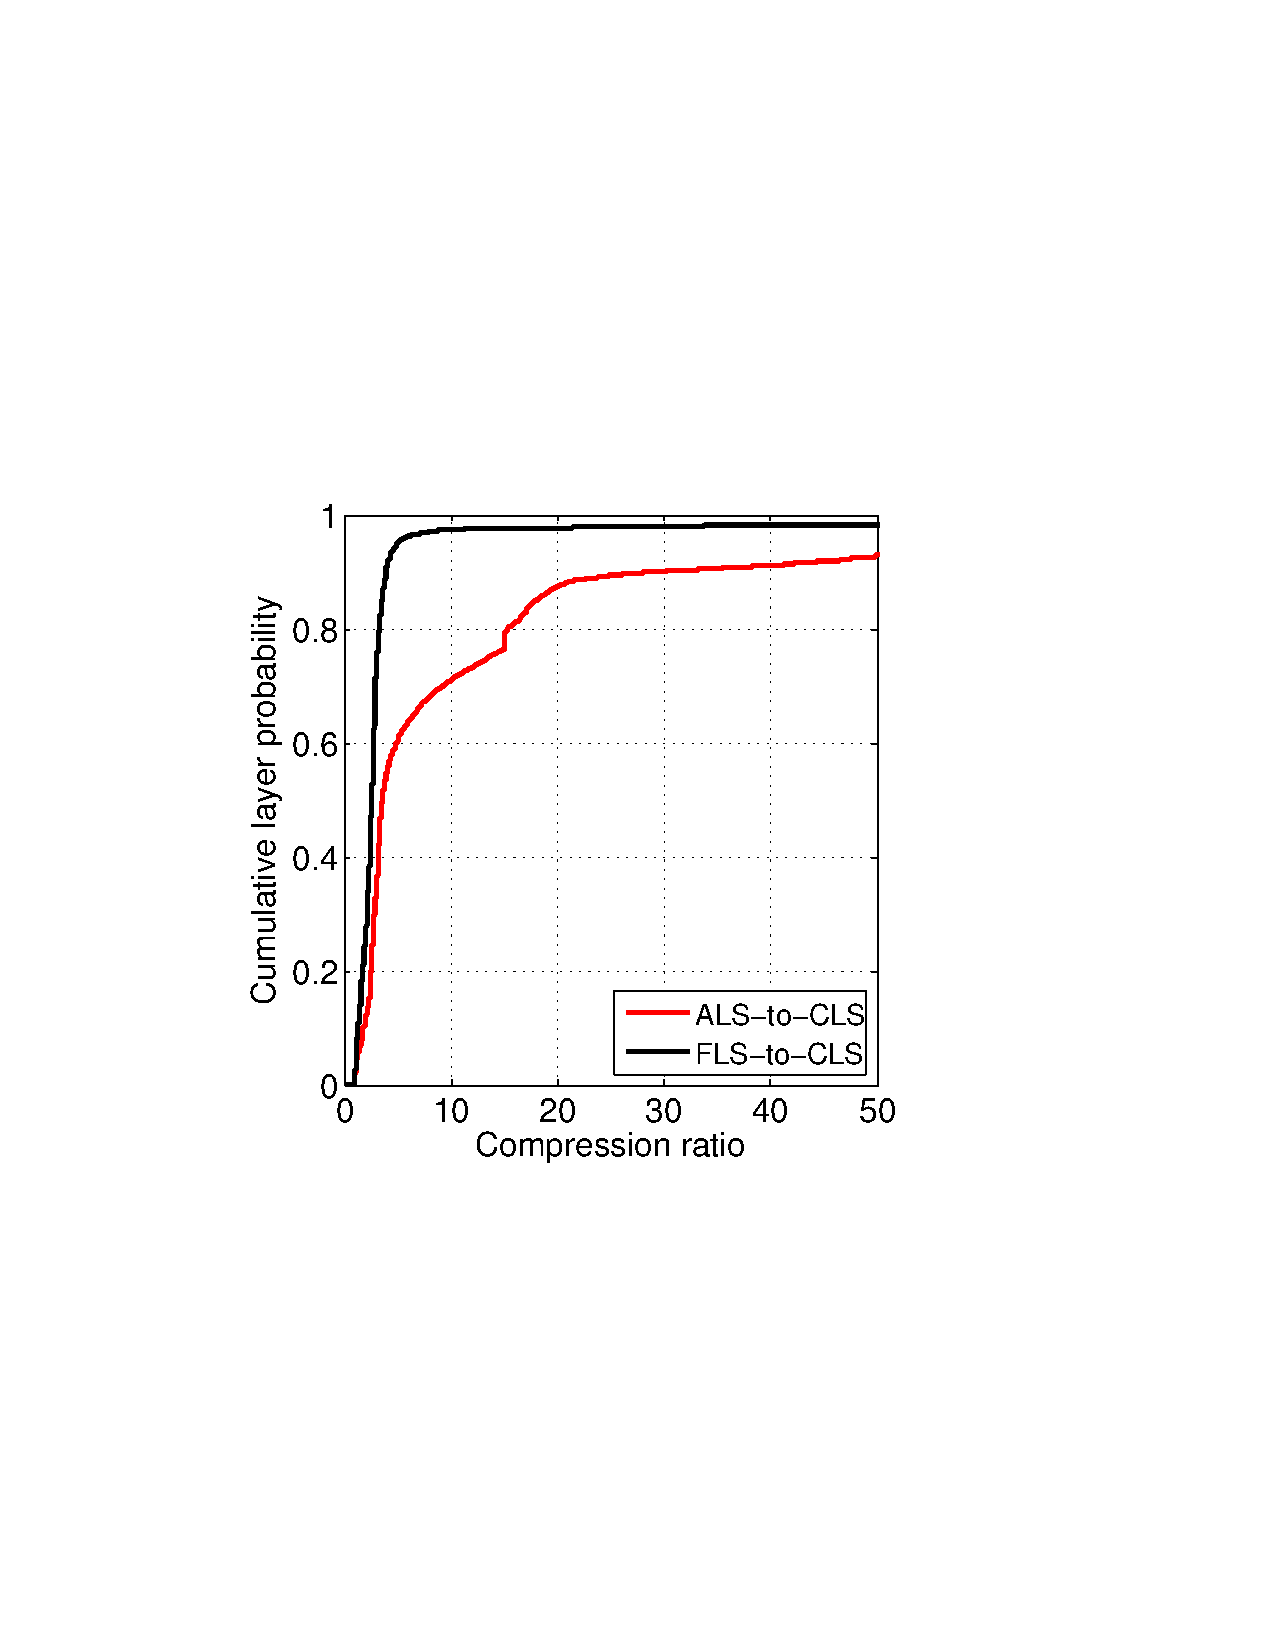
\includegraphics[width=0.23\textwidth]{graphs/cdf_compression_ratio.pdf}
%	}
%	\subfigure[Histogram of comp. ratios]{\label{fig_his_compression_ratio}
%		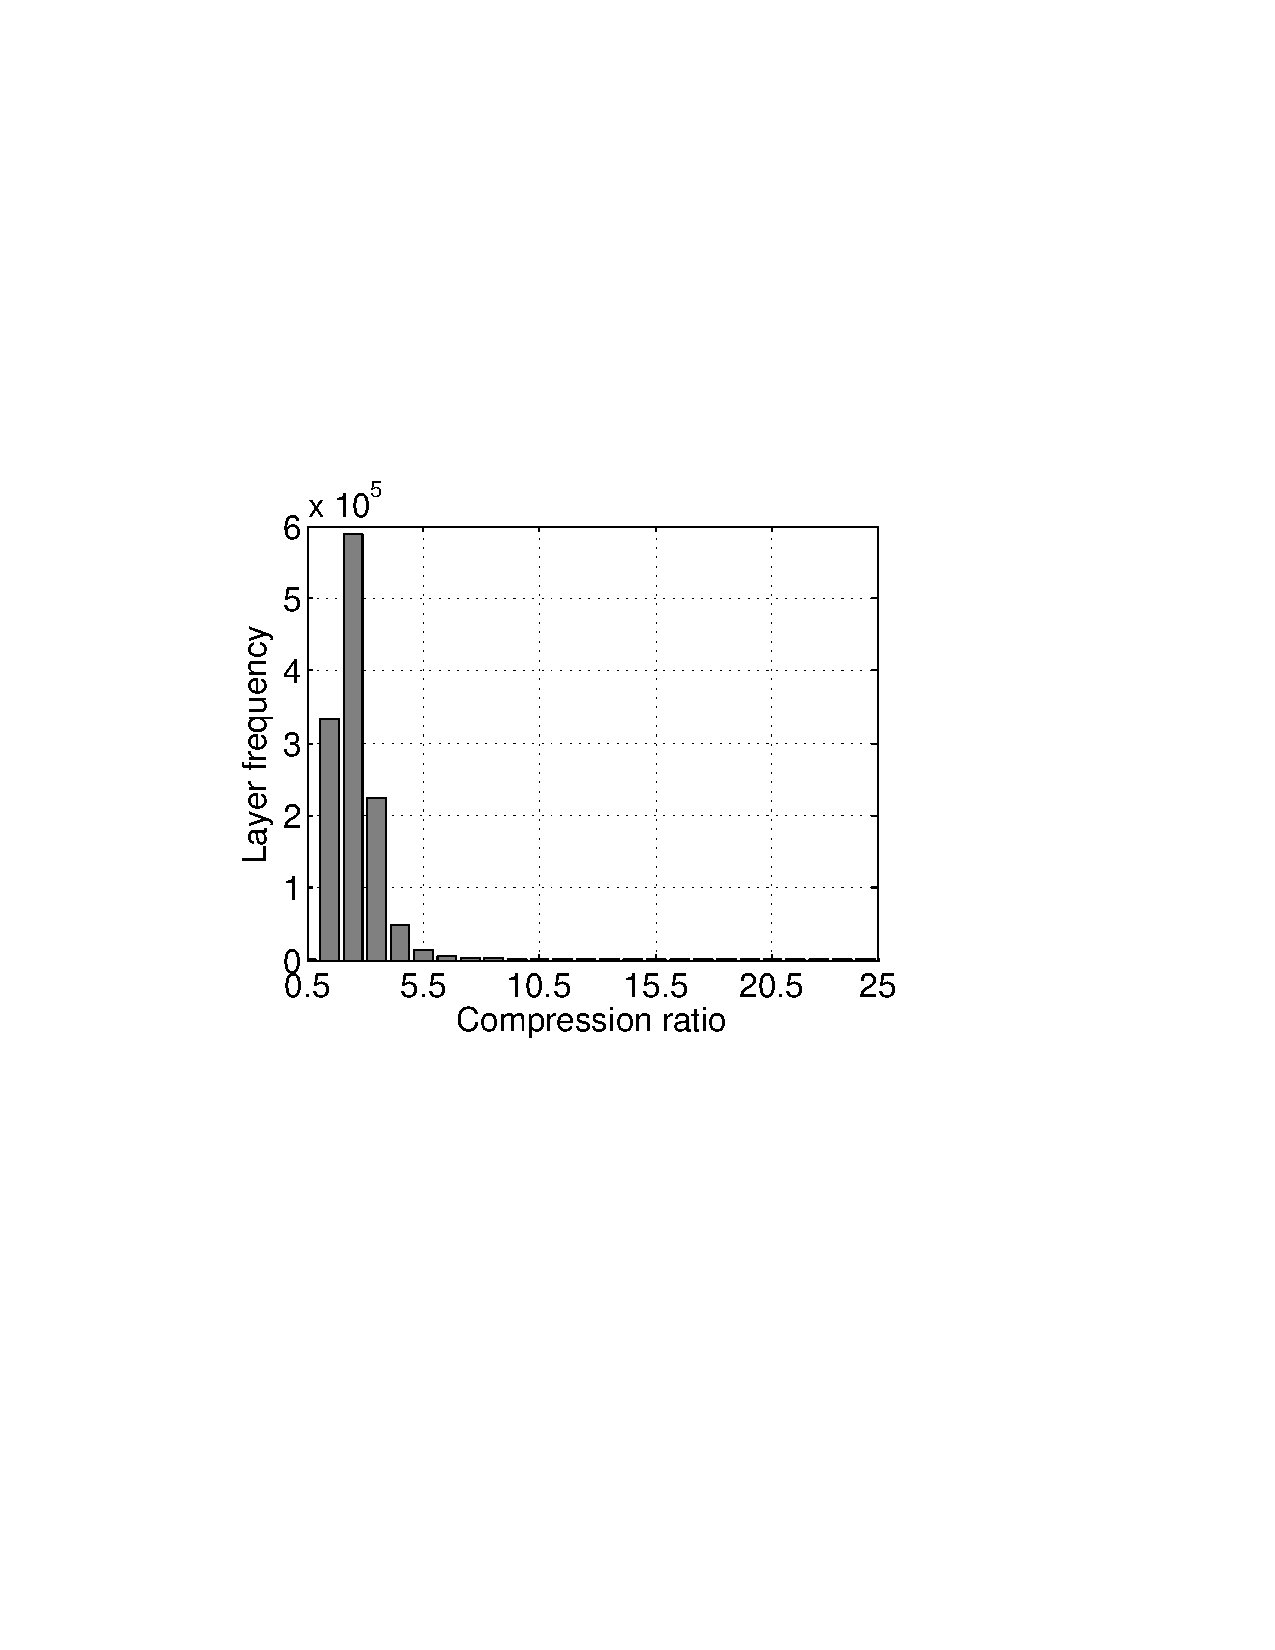
\includegraphics[width=0.223\textwidth]{graphs/his_compression_ratio.pdf}
%	}
%	\caption{Layer compression ratio distribution
%		%\vcomment{Different colors are used in figure (a) and (b) FLS/CLS\nancomment{will address later}}
%	}
%	\label{fig-compression-ratio}
%\end{figure}


%\begin{figure}[t]
%	\centering
%	\begin{minipage}{0.26\textwidth}
%		\centering
%		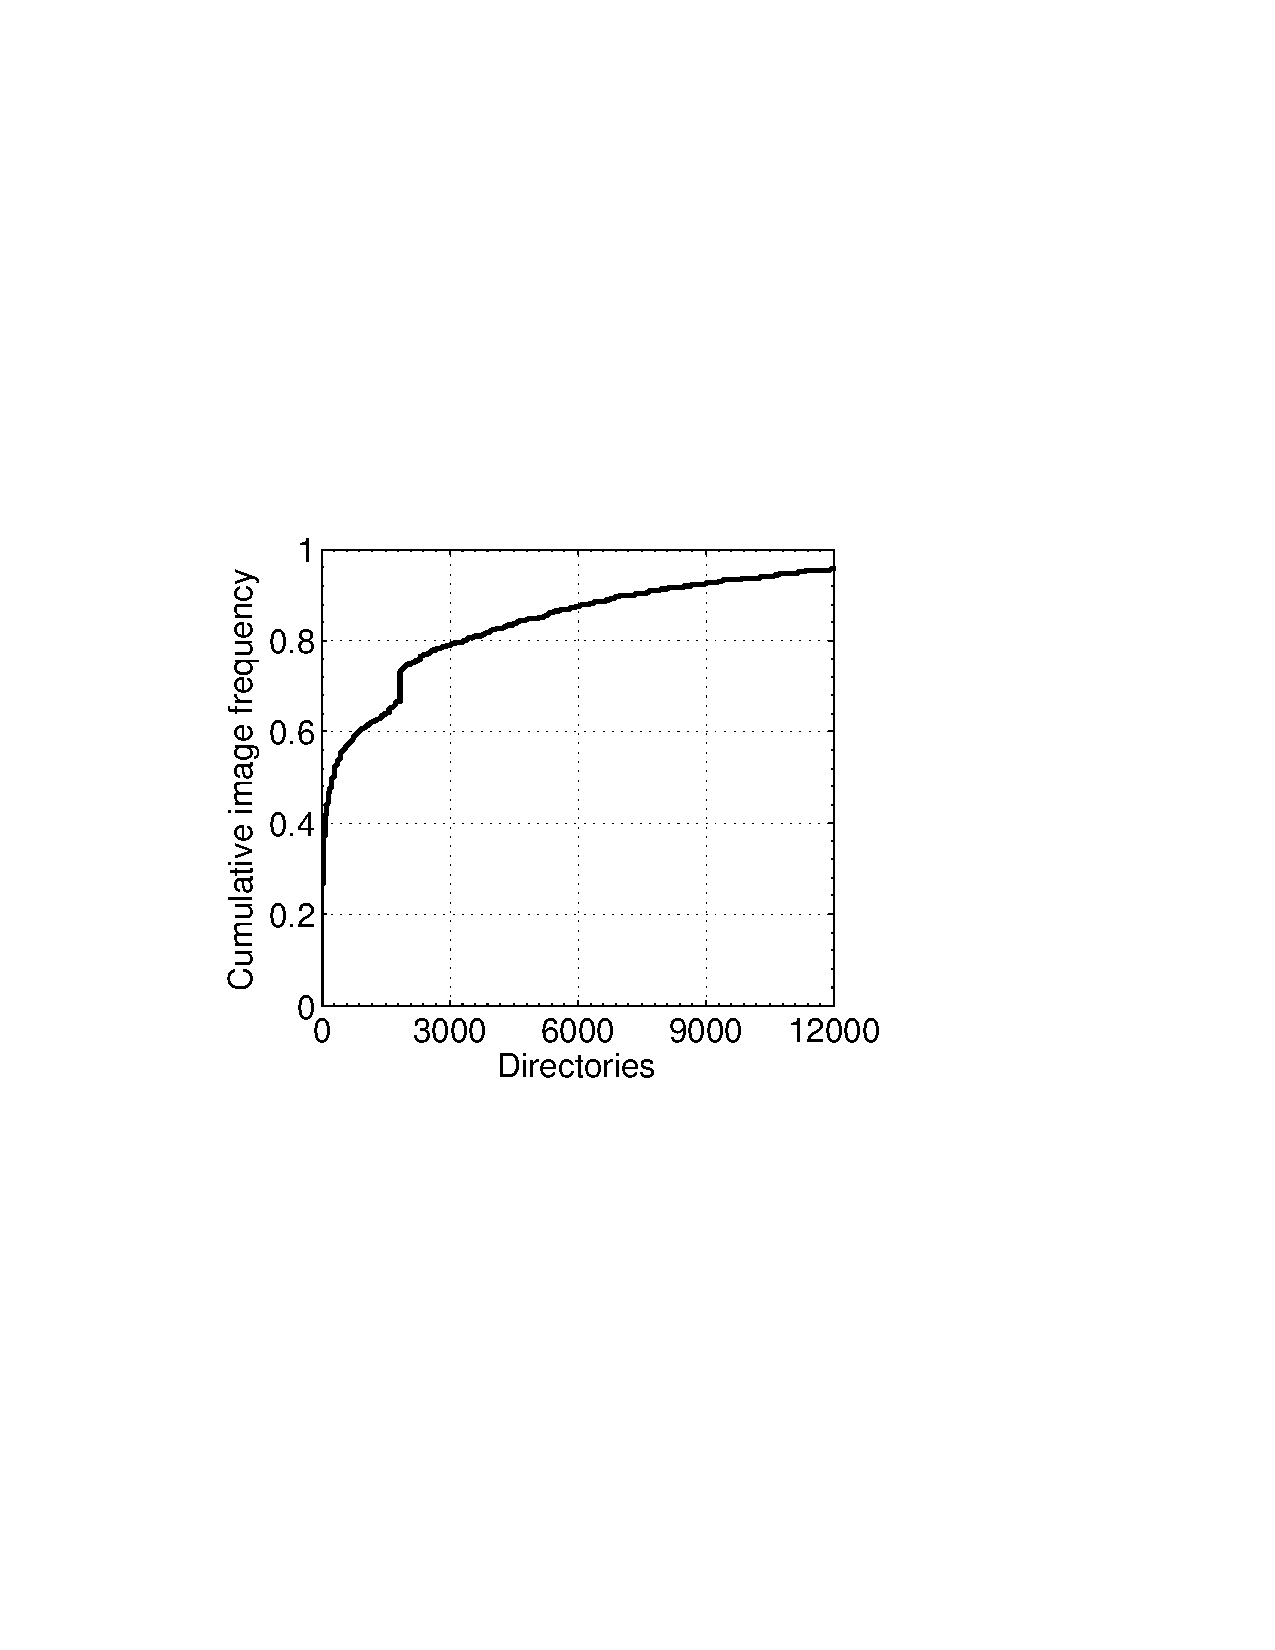
\includegraphics[width=1\textwidth]{graphs/dir.pdf}
%		\caption{CDF of images by\newline directories}
%		\label{fig-dir}
%	\end{minipage}%
%	\begin{minipage}{0.24\textwidth}
%		\centering
%		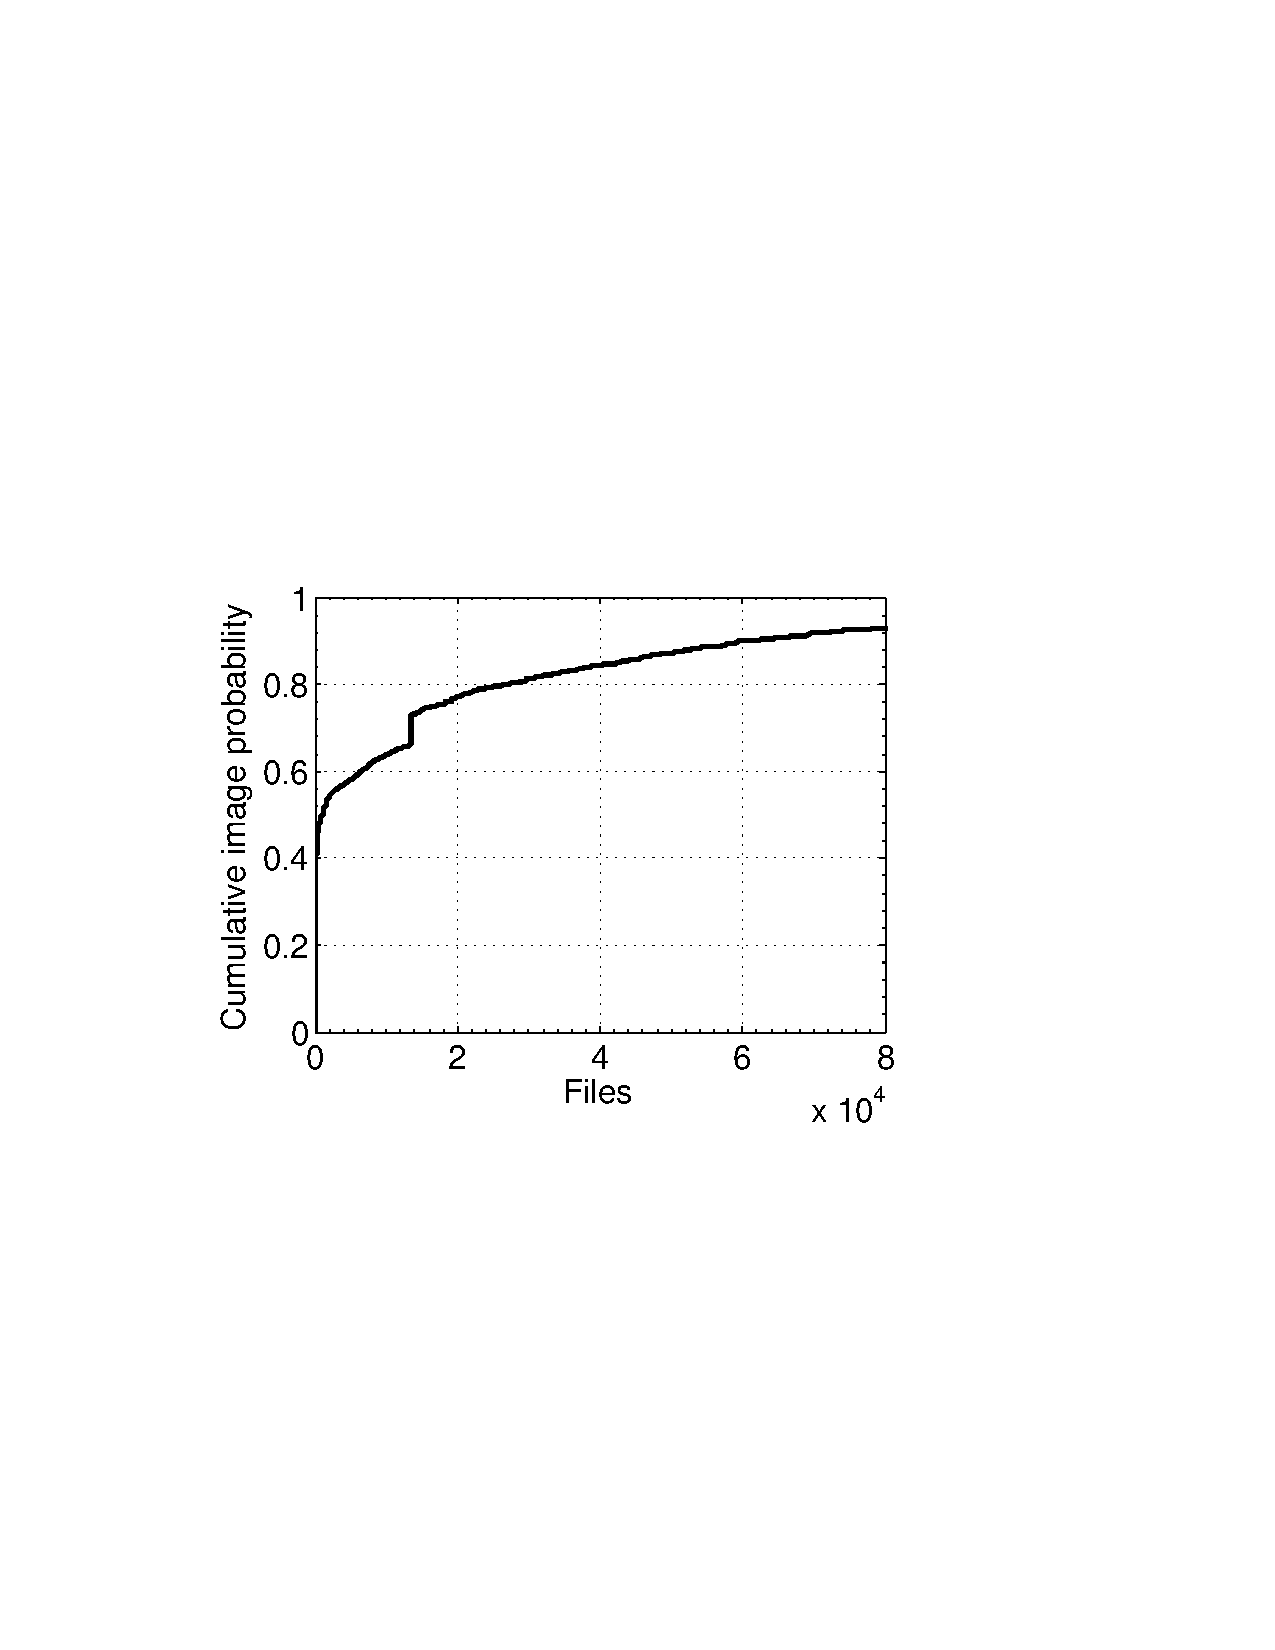
\includegraphics[width=1\textwidth]{graphs/file.pdf}
%		\caption{CDF of images by files}
%		\label{fig-file}
%	\end{minipage}
%\end{figure}

%\begin{figure}[htbp] 
%	\begin{minipage}{0.5\linewidth} 
%		\centering 
%		\includegraphics{circle} 
%		\caption{A Circle} 
%		\label{fig:circle} 
%	\end{minipage}% 
%	\begin{minipage}{0.5\linewidth} 
%		\centering 
%		\includegraphics{rectangle} 
%		\caption{A Rectangle} 
%		\label{fig:rectangle} 
%	\end{minipage} 
%\end{figure}


Figure~\ref{fig:layer-repull-cdf} shows the CDF of layer repull count. Here, \emph{repulling} indicates the act of pulling layers that have been pulled by the user before because they are no longer present on the user side.
We see that majority of users don't \emph{repull} layers frequently.
For \texttt{Syd}, only 4\% of layers are repulled by the same clients.
\texttt{Dev} has the highest repull layer ratio of 36\% while 83\% of the repull layers are only repulled twice.
Majority of repulled layers are repulled infrequently.
For example, only 3\% of layers from \texttt{Syd} are repulled more than twice.
Layer from \texttt{Prestage} and \texttt{Lon} have the highest repull frequency.
5\% of layers are pulled more than 6 times.
We also observe that few clients \emph{repull} layers continuously.
The highest layer repull count is 19,300 from \texttt{Lon}.
We think these clients probably deploy containers on a shared platform such as Cloud,
and run ephemeral jobs such as stateless microservices. 
Once the applications are finished, the container images are automatically deleted.
So when users launch containers again, they will repull layers again.

When different clients \texttt{pull} the same repository, 
they will fetch different amount of layers from the repository based on the contents of their local layer dataset.
Even when the same clients \texttt{pull} the same repository at different times, 
they will fetch different amount of layers from the repository because their local layer dataset changes over time.
Therefore, a \texttt{pull manifest} requests doesn't usually result in repulling the layers in the repository. 
Here, we define \emph{repulling a repository} as repulling the layers in the repository for the same client.
Figure~\ref{fig:repo-repull-cdf} shows the CDF of the probability of repository repulling.
The probability of repository repulling is calculated 
as the number of \texttt{pull manifest} resulting in repository repulling divided by 
the total number of \texttt{pull manifest} requests issued by the same client for the same repository.
We see that majority of repositories aren't repulled.
The repull repository ratio ranges from 15\% for \texttt{Prestage} to 43\% for \texttt{Prestage}.
Majority of repull repositories have a low repulling probability.
Only 20\% of repositories from  \texttt{Prestage}, \texttt{Stage}, and 
\texttt{Syd} have a repulling probability higher than 0.5.
And only 20\% of repositories from the rest 4 workloads have a repulling probability higher than 0.33.
We also observe that few repositories' repulling probability are 1, meaning 
every time clients pull these repositories, they always repull the layers in these repositories. 
 
Figure~\ref{fig:client-repull-cdf} shows the client repulling probability.
Client repulling probability is calculated as the number of \emph{repull} layer requests divided by
the number of all \texttt{pull} layer requests issued by the same client.
We see that majority of clients do repull layers but the probability is low.
60\% of clients from \texttt{Prestage}, \texttt{Dev}, \texttt{Lon}, and \texttt{Fra} have a repulling probability lower than 0.1.
55\% of clients from both \texttt{Dal} and \texttt{Stage} have a repulling probability lower than 0.1.
Less clients have repulling probability range between 0.1 to 0.7.
10\%-30\% of clients have a repulling probability ranged from 0.2-0.7 across 7 workloads.
We find few clients repull layers continuously.
2\%-12\% of clients have a repulling probability higher than 0.9 from workloads:
\texttt{Dal}, \texttt{Dev}, \texttt{Fra}, \texttt{Prestage},
\texttt{Stage}, \texttt{Syd}, and \texttt{Lon}.

%\paragraph{Monitor user access patterns}
%To monitor user access patterns,
%\preconstructcachename~first uses a RLmap to record repository-layer relationship.
%If user~\emph{u} \emph{pushes} a  layer~\emph{l} to a repository~\emph{r},
%\preconstructcachename~will add an new entry (\emph{l}) in RLmap denoted as RLmap[\emph{r, l}]. 
%%Based on user access patterns,
%\preconstructcachename~ also maintains a URLmap for keeping track of user access patterns.
%To identify a user, 
%we extract \emph{user end host address} (\emph{r.client}) from each request (\emph{r}). 
%Each URLmap entry maintains a user profile for each user \emph{u} denoted as URLmap[\emph{u}]. %as shown in Figure~\ref{xxx}.
%User profile contains a list of repository profiles for each accessed repository \emph{repo} denoted as URLmap[\emph{u, repo}],
%and each repo profile contains a list of layer profiles for each accessed layer \emph{l}  denoted as URLmap[\emph{u, repo, l}].
%Note that layer profiles can be shared among different repo profiles for the same user.
%If user~\emph{u} \texttt{pull}s a layer~\emph{l} from a repository~\emph{repo},
%\preconstructcachename will update layer profile URLmap[\emph{u, repo, l}] with the corresponding layer repull count, and calculate
%repository repulling probability and user repulling probability for the corresponding repository profile and user profile.
%Each node records the following history information: (\emph{Get\_cnt}, \emph{Put\_cnt}, \emph{last\_access\_time}). a child node layer~\emph{L} to parent node~\emph{R}
%User profile records the user repulling probability $u.rp$ for client $u$.
%If $u.rp$ is greater than threshold $\theta_{crp}$, this user has a high probability of repulling layers.
%Repo profile records repository repulling probability $u.r.rp$ for repository $r$.
%If $u.r.rp$ is greater than threshold $\theta_{rrp}$, this repository is a popular repulling repository for this user.
%Layer profile records layer repull count $u.l.R$ for layer $l$.
%If $u.l.R$ is greater than threshold $\theta_{R}$, this layer is a popular repull layer for this user.



%\subsubsection{User access pattern  based cache replacement}

%
%\preconstructcachename~starts cache eviction when free space is low.
%To decide which layer or slices need to be evicted to make space for new requests,
%we analyze the temporal trend of user accesses as follows.

\subsection{Skewness and temporal access patterns}
%\begin{figure*}[t]
%		\begin{minipage}{0.32\linewidth}
%			\centering
%			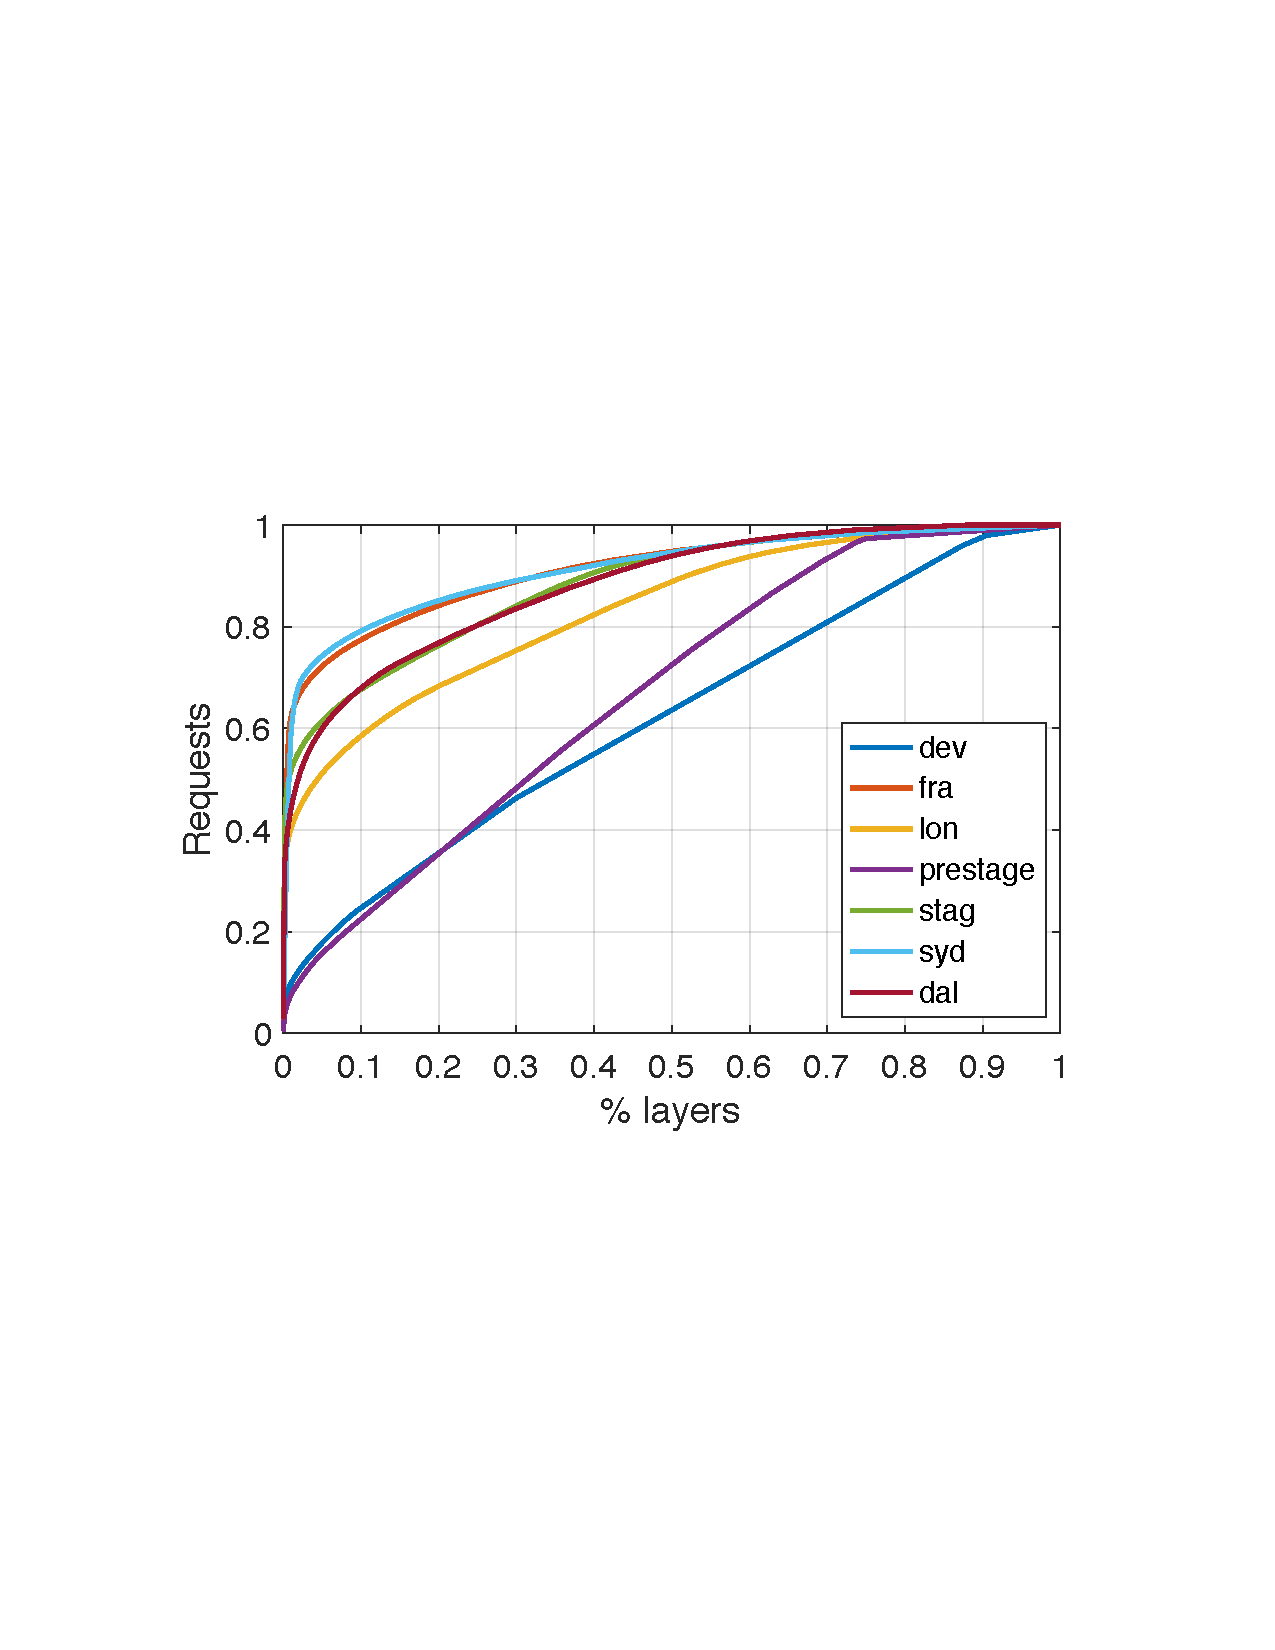
\includegraphics[width=1\textwidth]{graphs/layer_skewness.pdf}
%			%\caption{CDF of layer  count.}
%		%	\vspace{-3pt}
%			\label{fig:layer-skenwess}
%		\end{minipage}
%			\begin{minipage}{0.32\linewidth}
%				\centering
%				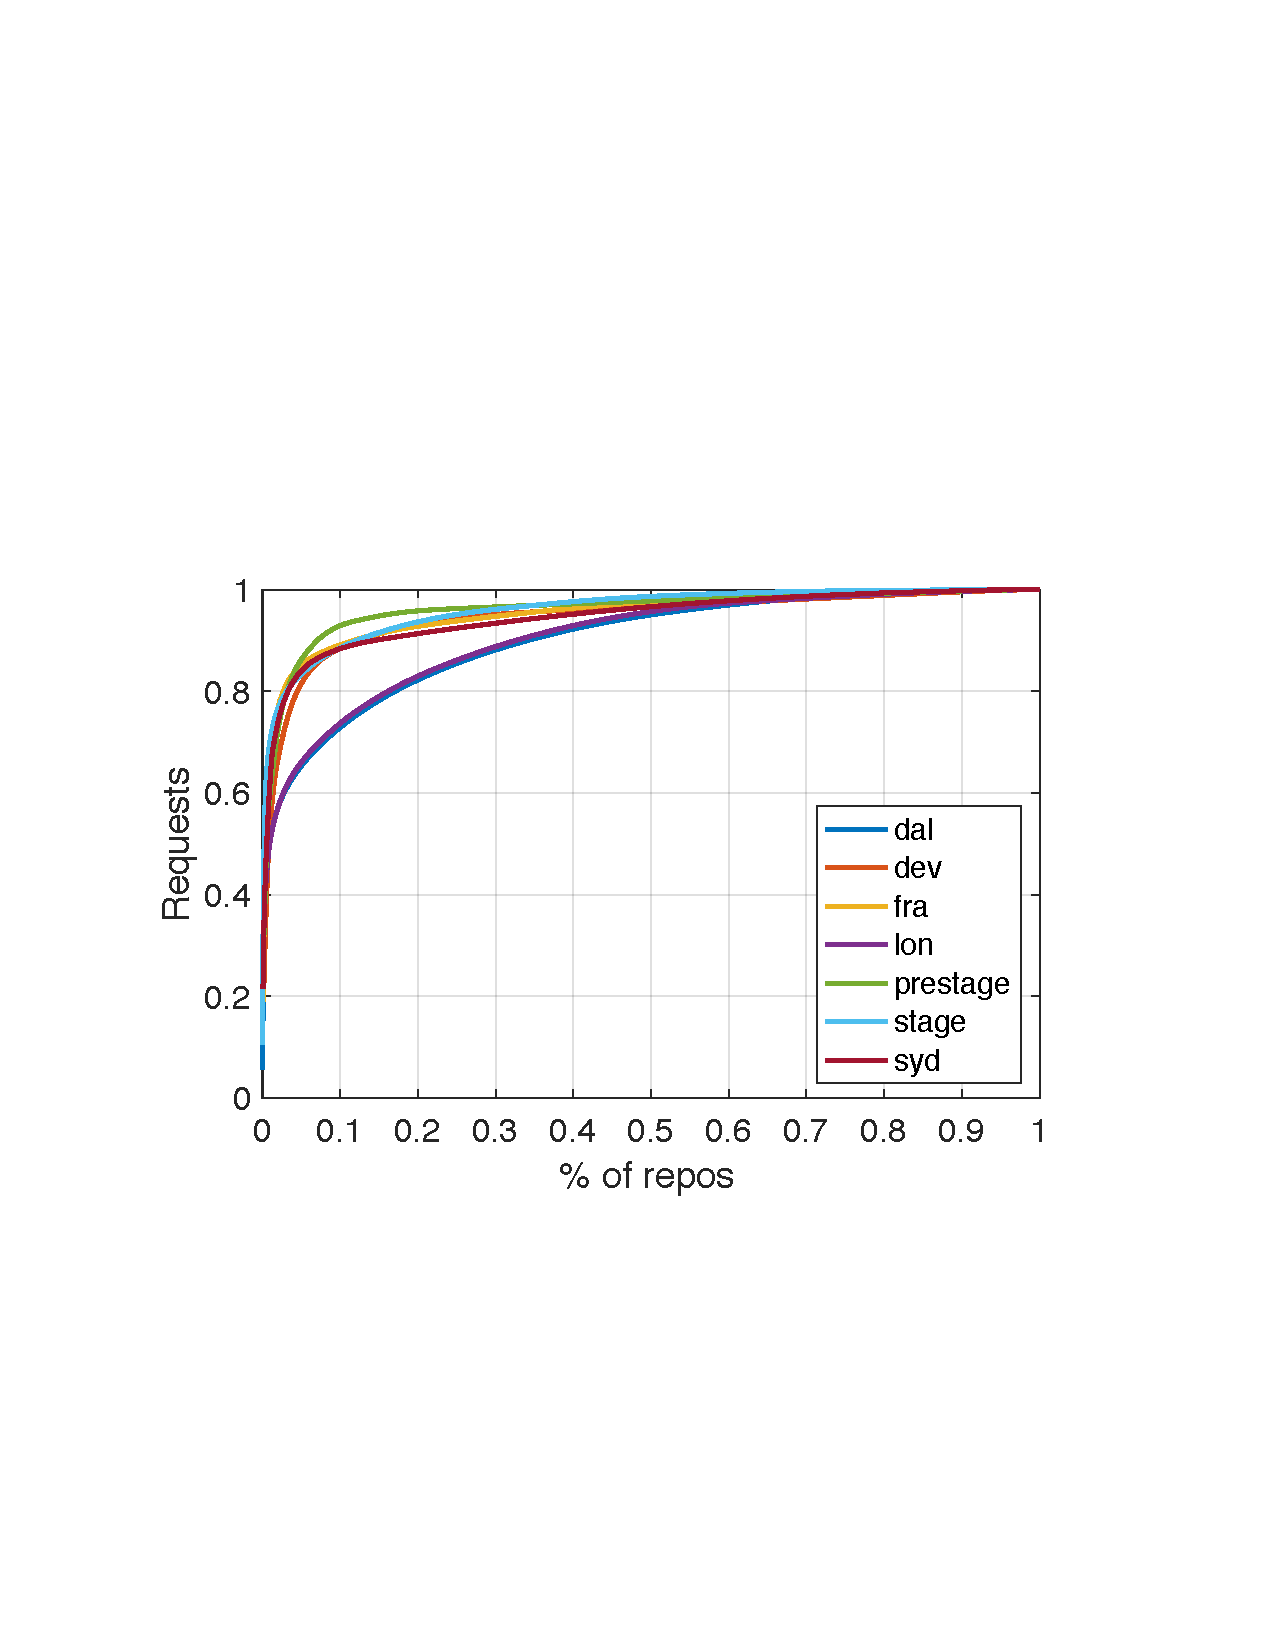
\includegraphics[width=1\textwidth]{graphs/repo-skewness.pdf}
%				%\caption{PDF of repository repulling probability.}
%				%	\vspace{-3pt}
%				\label{fig:repo-skewness}
%			\end{minipage}
%		\hfill
%		\begin{minipage}{0.32\linewidth}
%			\centering
%			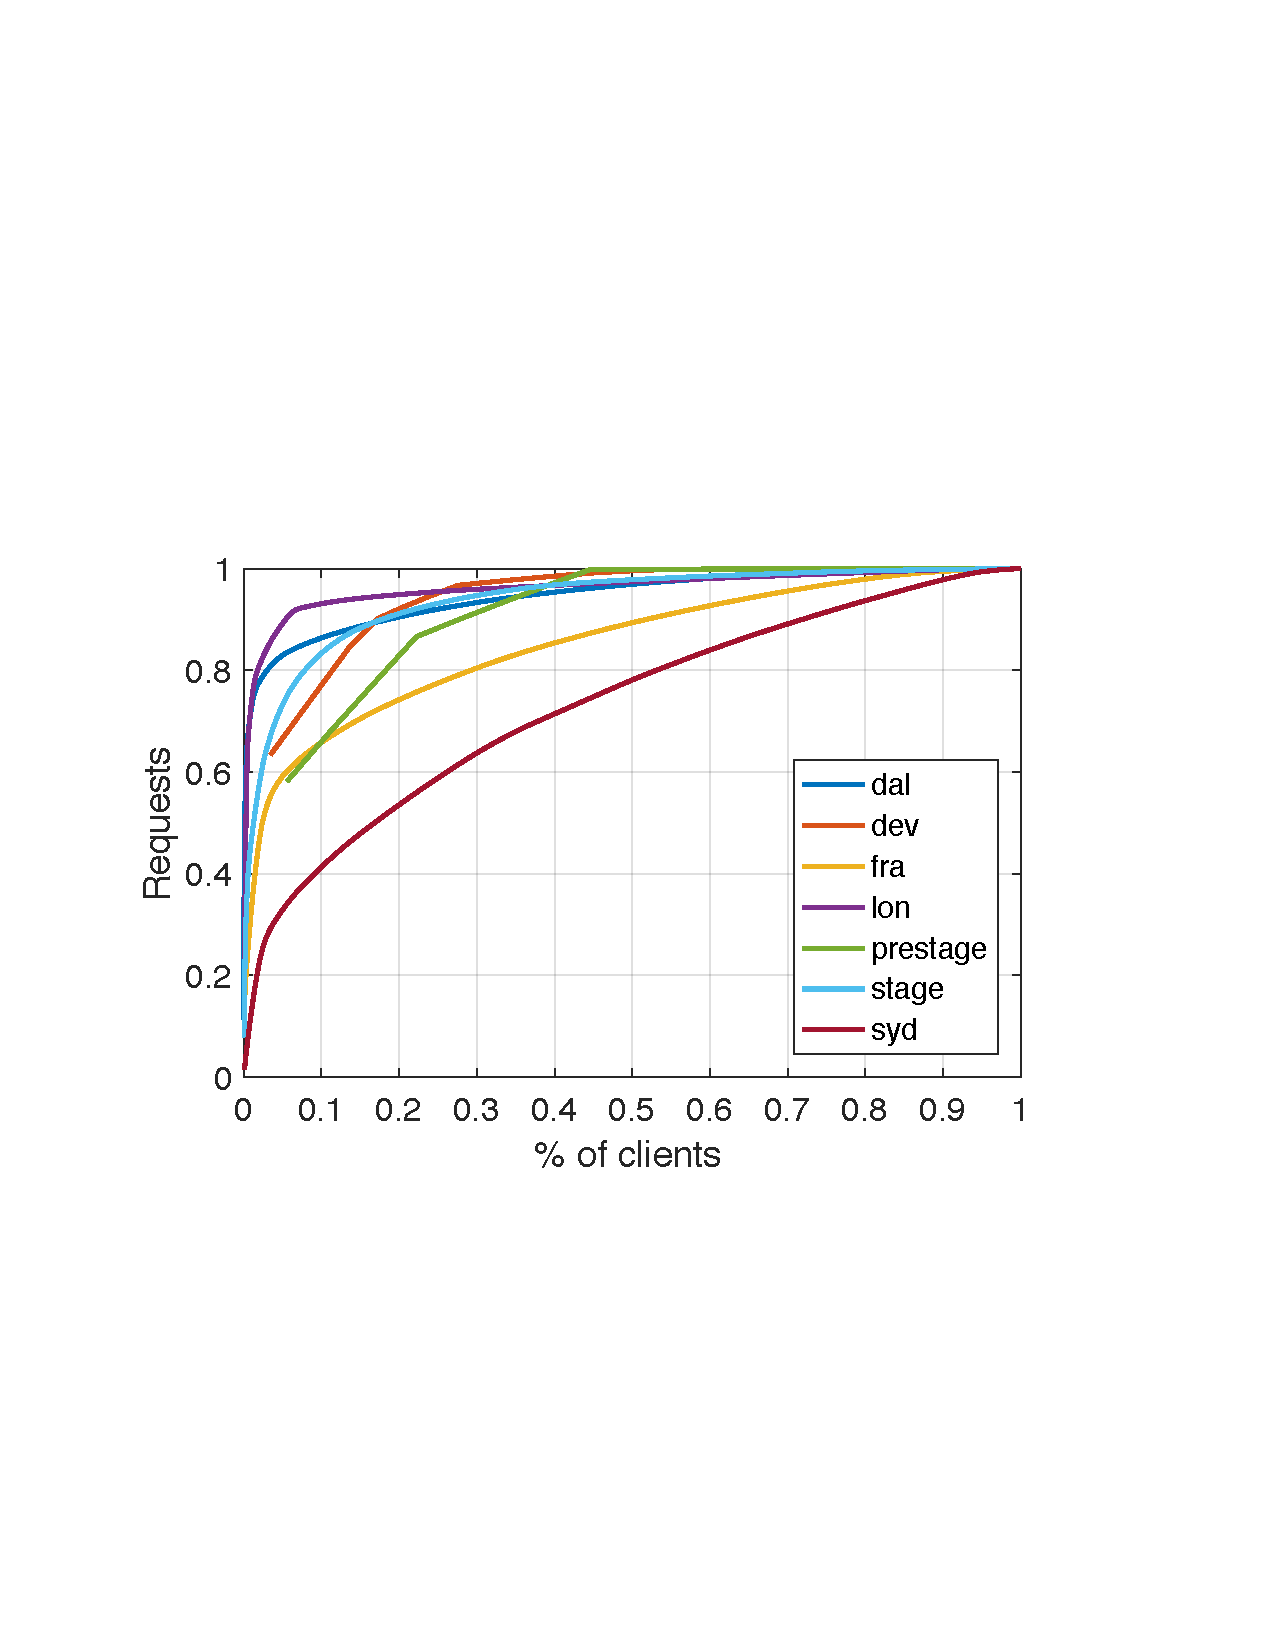
\includegraphics[width=1\textwidth]{graphs/client-skewness.pdf}
%			%\caption{PDF of client repulling probability.}
%			%	\vspace{-3pt}
%			\label{fig:client-skewness}
%			
%		\end{minipage}
%\caption{PDF of probability for layers, repositories, and clients.}
%%	\label{}
%\end{figure*}

\begin{figure*}[!t]
	\centering
	\subfigure[Layer repull count]{
		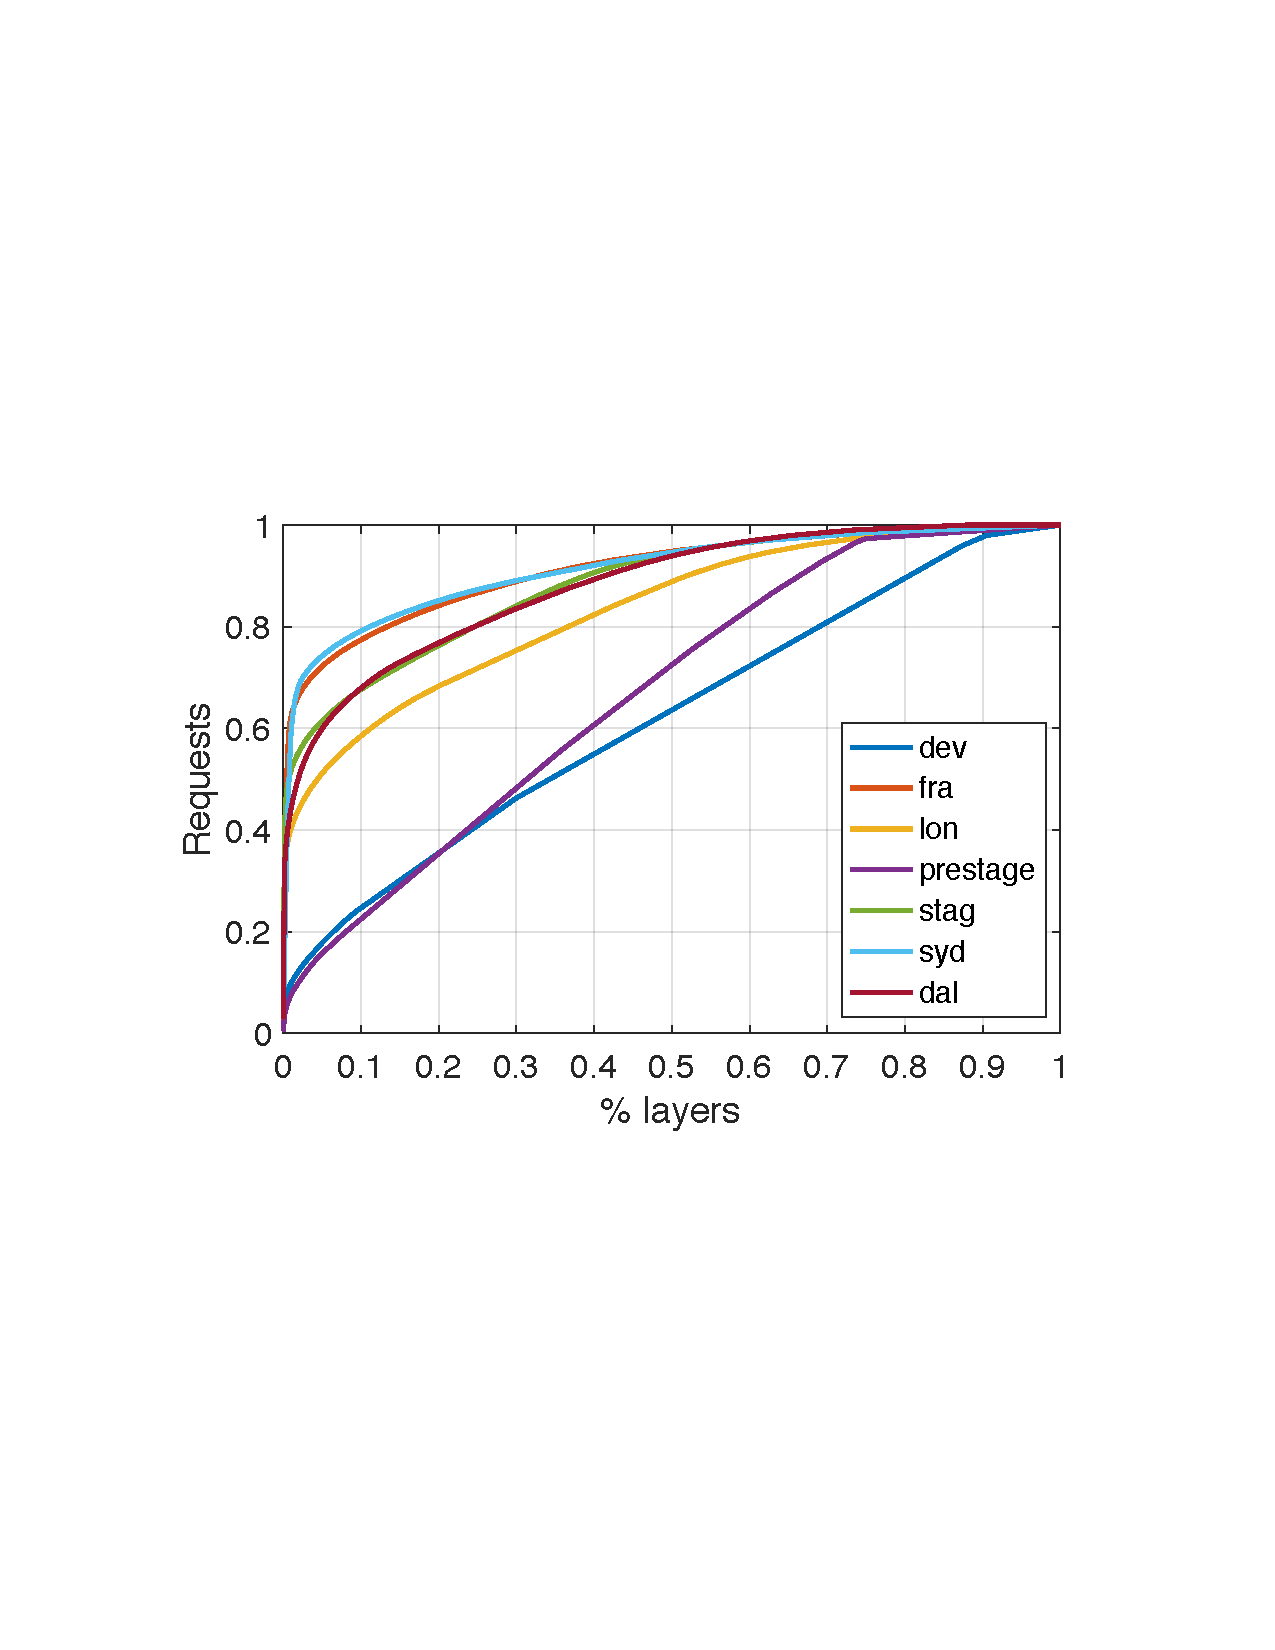
\includegraphics[width=0.2\linewidth]{graphs/layer_skewness.pdf}
		\label{fig:layer-skenwess}
	}
	\subfigure[Repository repulling probability]{
		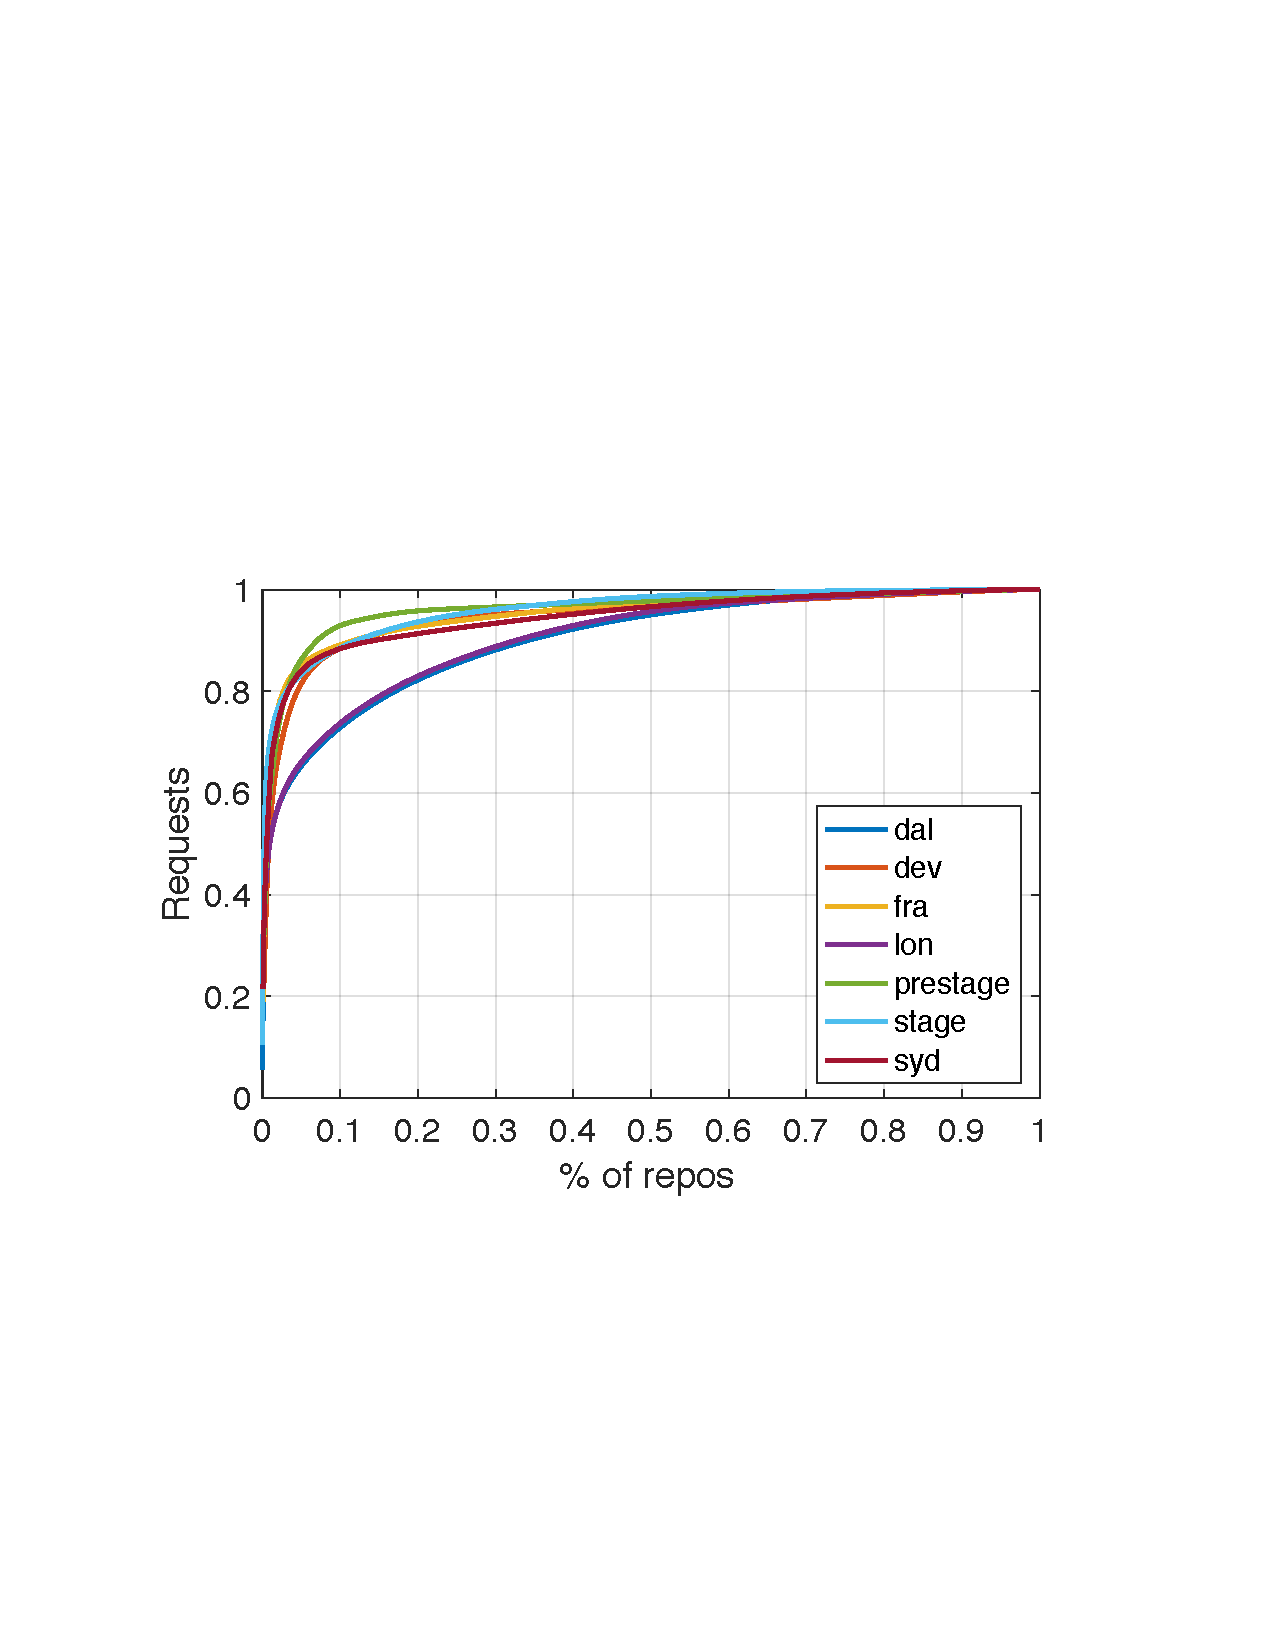
\includegraphics[width=0.2\linewidth]{graphs/repo-skewness.pdf}
		\label{fig:repo-skewness}
	}
	\subfigure[Client repulling probability]{
		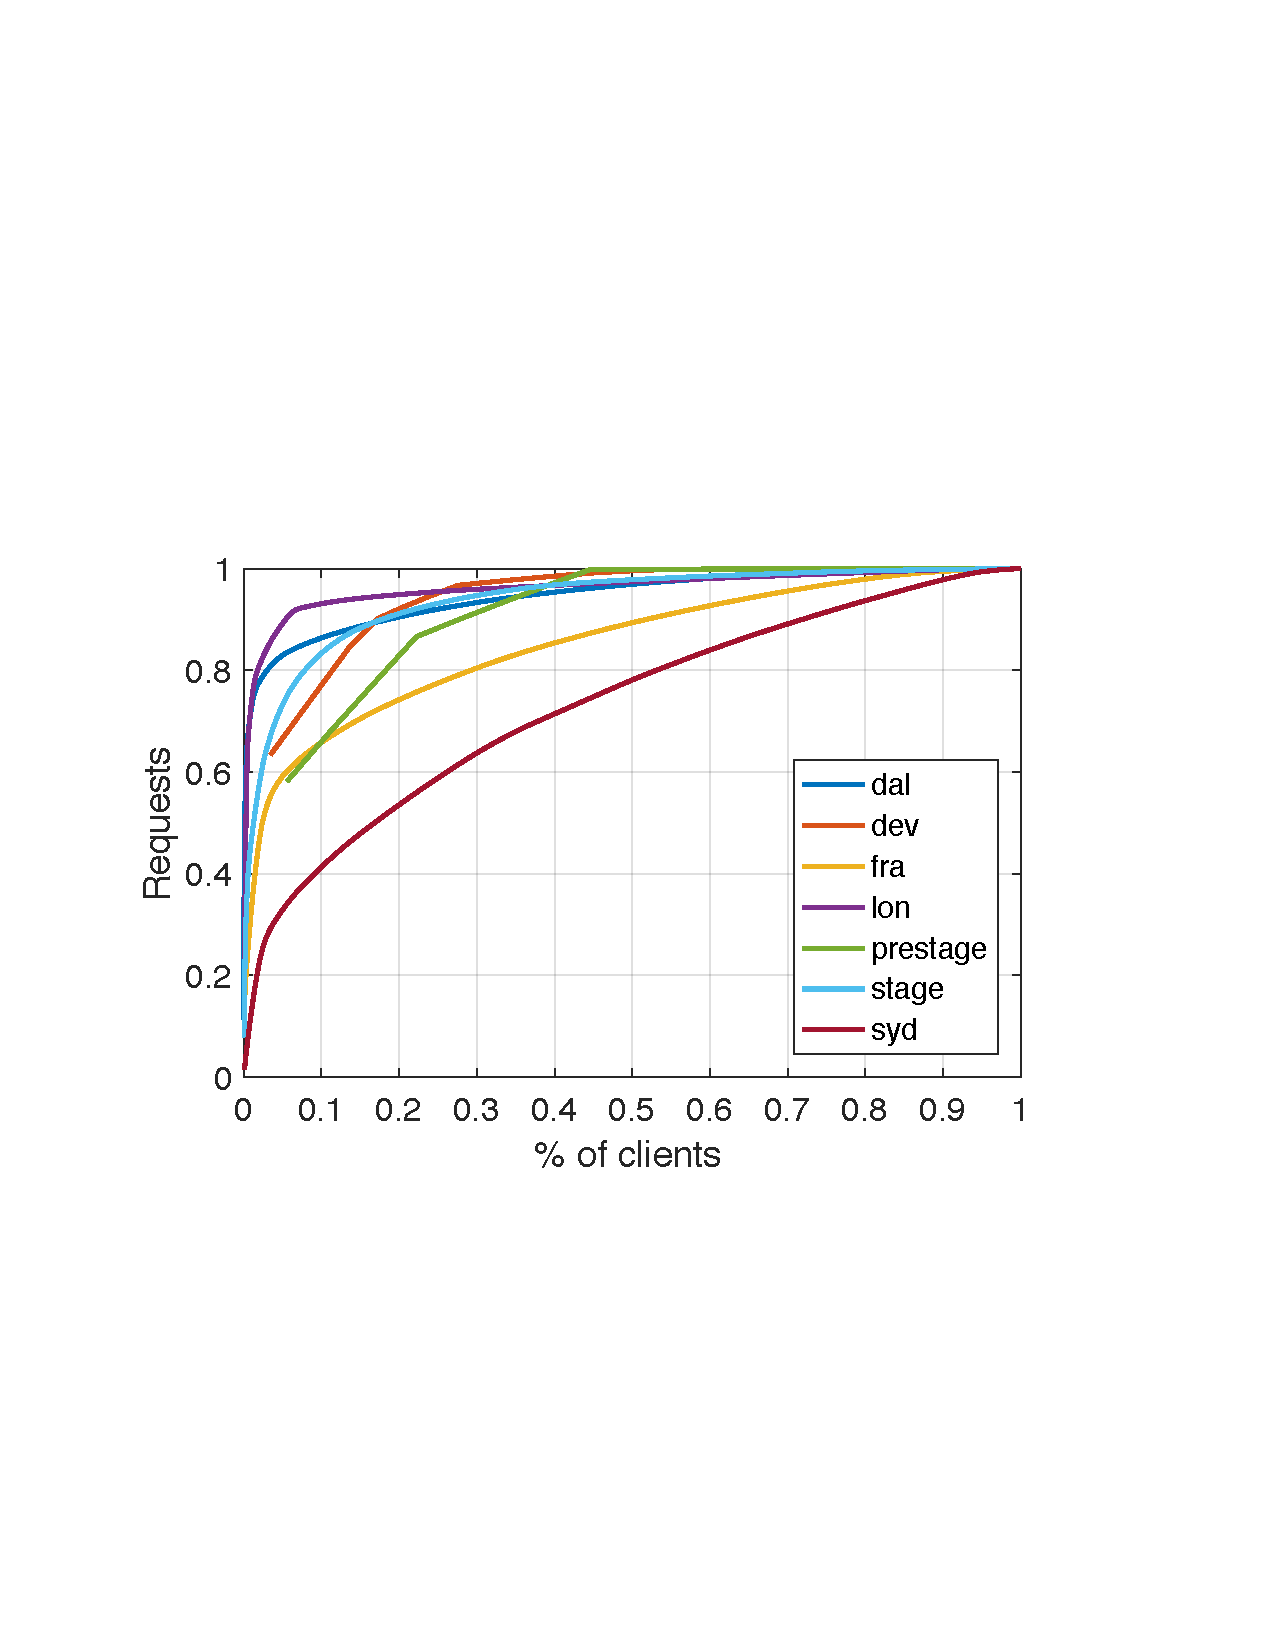
\includegraphics[width=0.2\linewidth]{graphs/client-skewness.pdf}
 	\label{fig:client-skewness}
	}
\caption{PDF of probability for layers, repositories, and clients.}
	\label{fig-skewness}
\end{figure*}
%\begin{figure*}[t]
%		\begin{minipage}{0.32\linewidth}
%			\centering
%			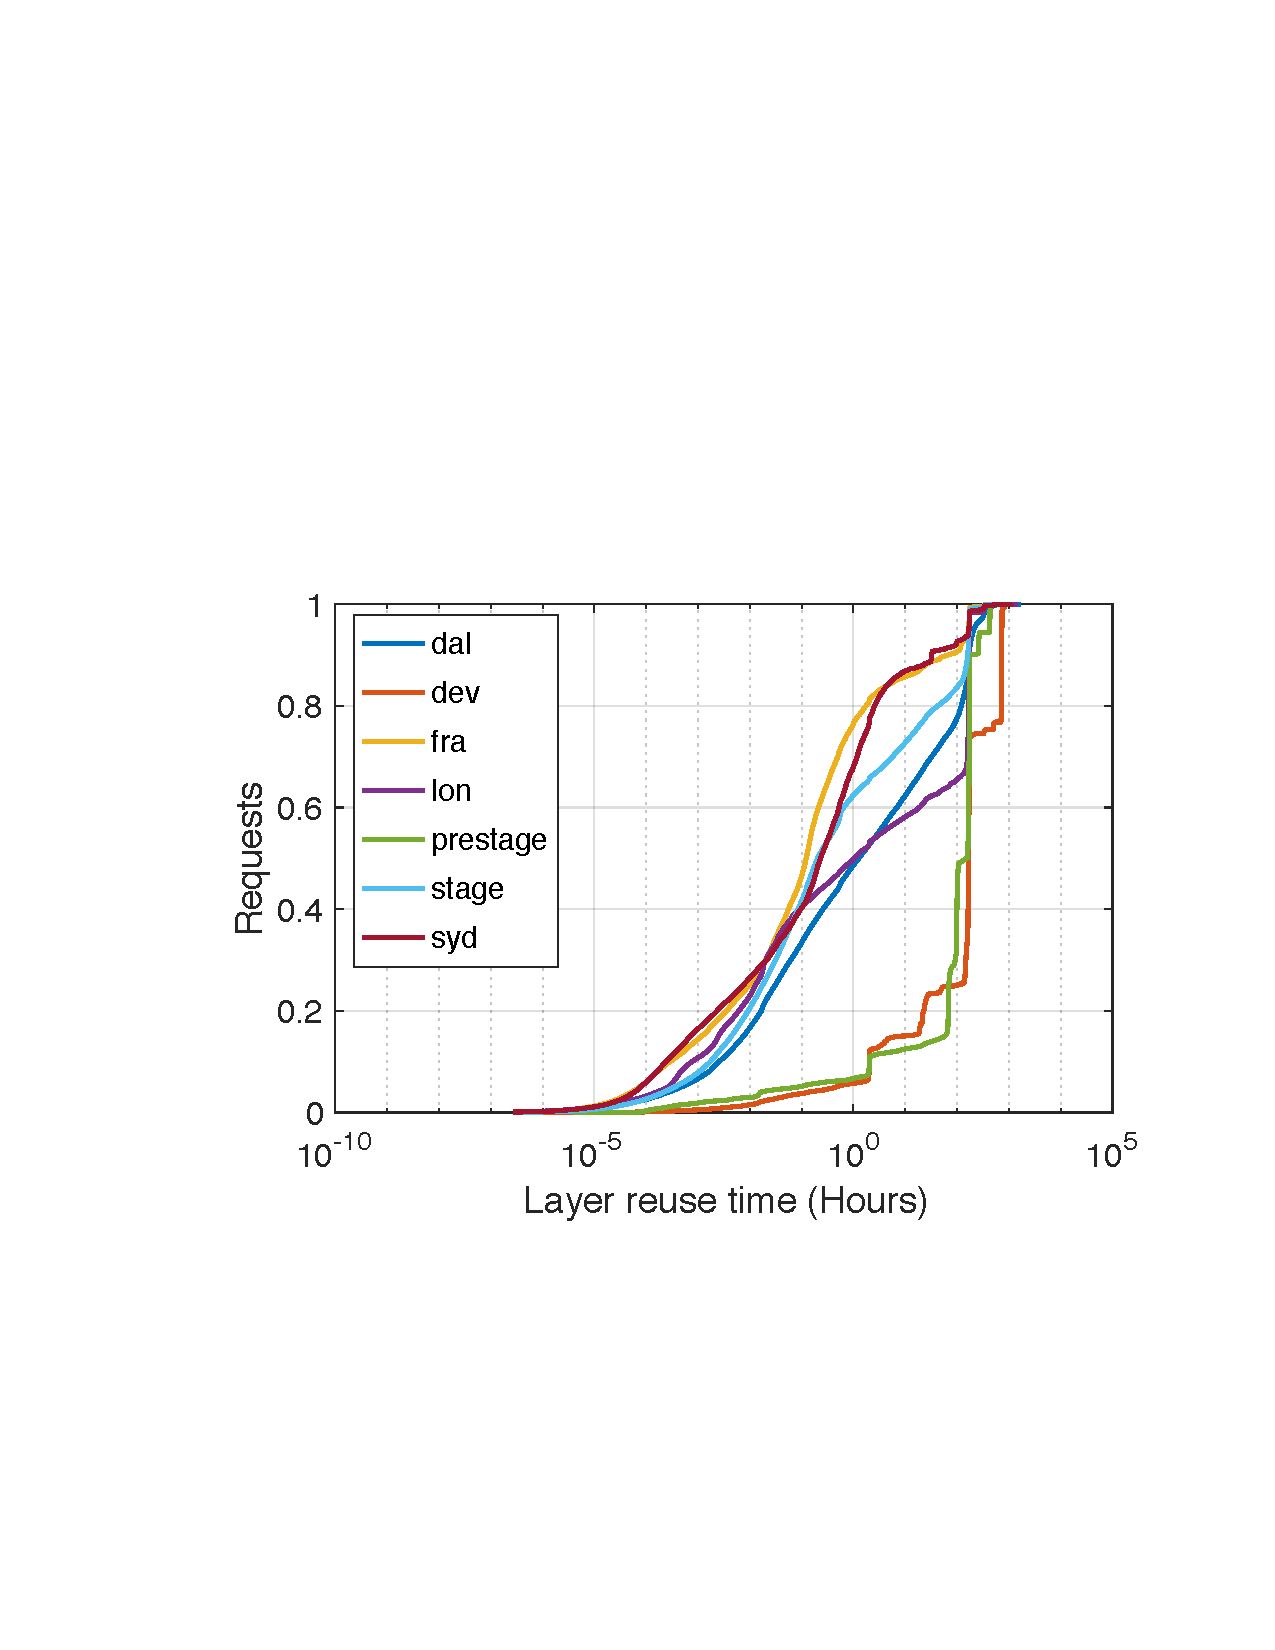
\includegraphics[width=1\textwidth]{graphs/layer-reusetime.pdf}
%		%	\caption{CDF of layer reuse time.}
%		%	\vspace{-3pt}
%			\label{fig:layer-reuse}
%		\end{minipage}
%			\begin{minipage}{0.32\linewidth}
%				\centering
%				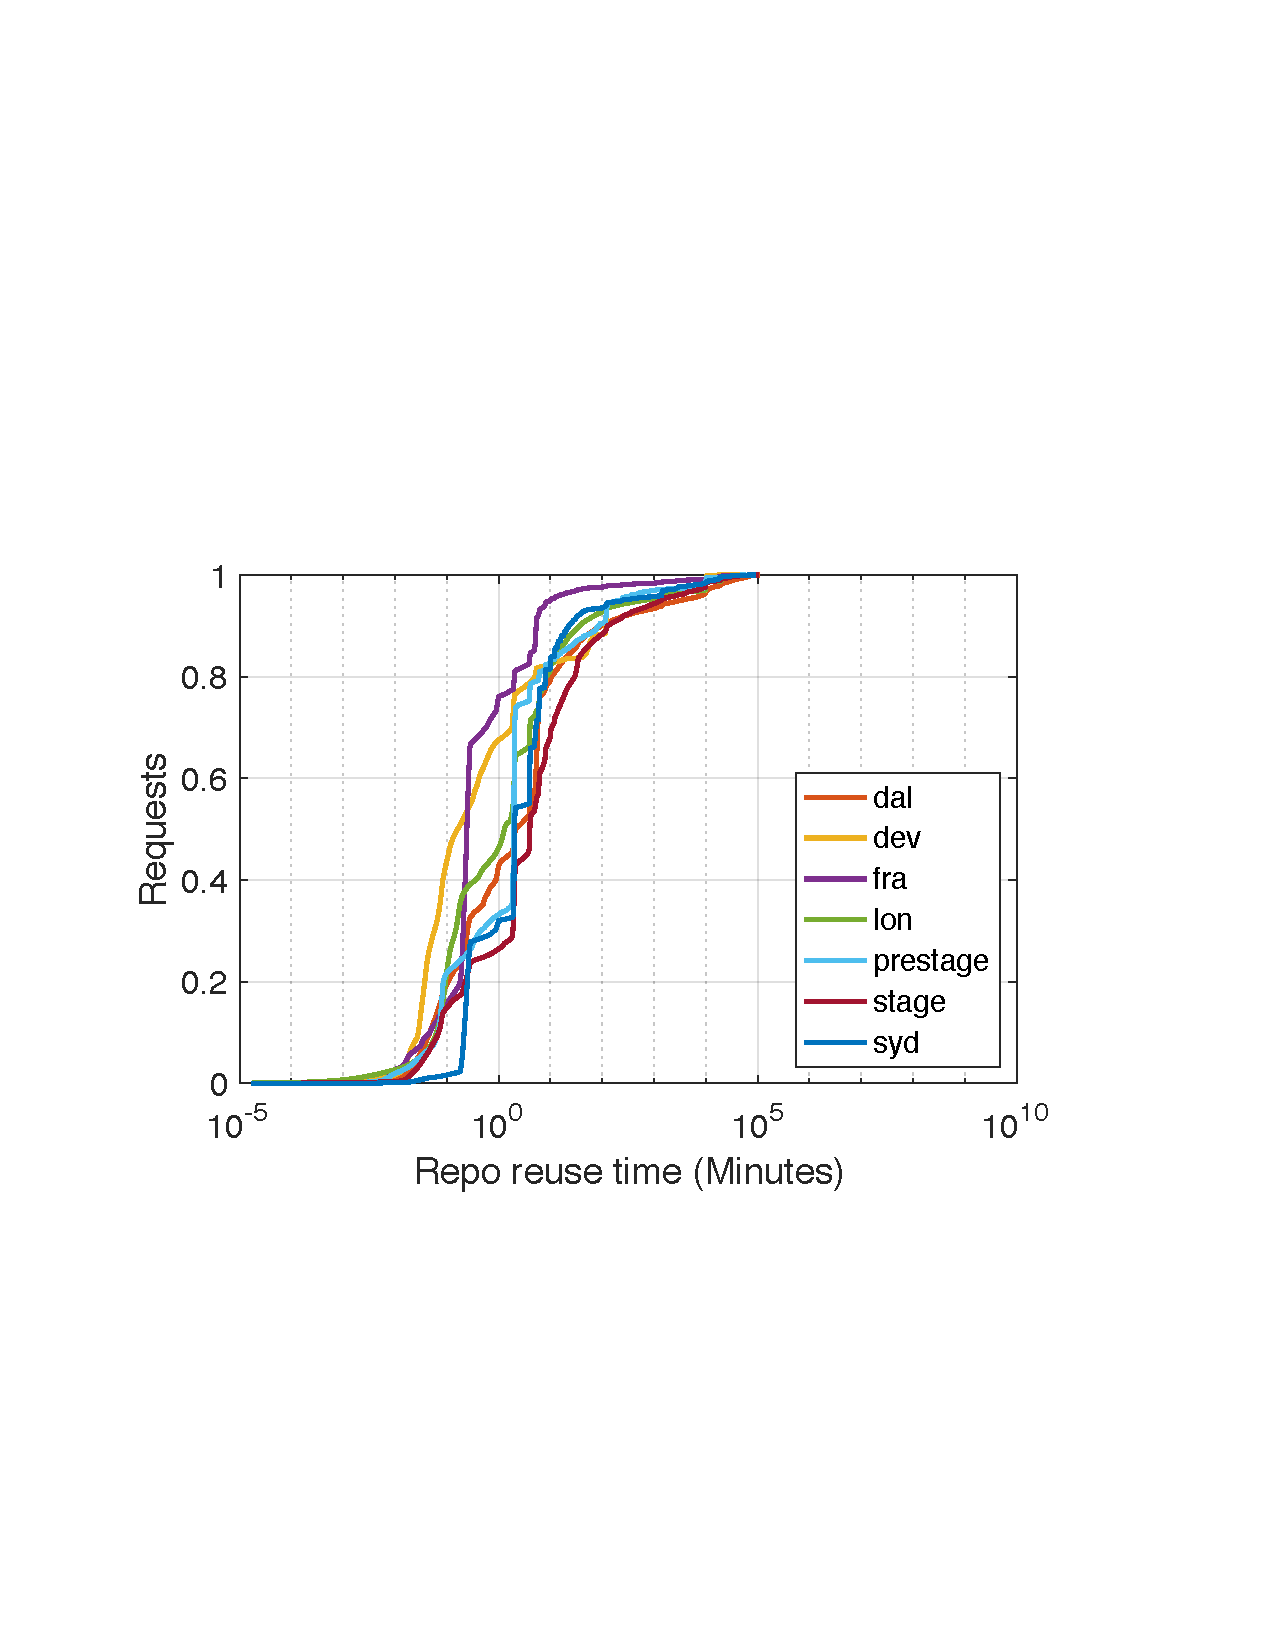
\includegraphics[width=1\textwidth]{graphs/repo-reusetime.pdf}
%			%	\caption{PDF of repository reuse time.}
%				%	\vspace{-3pt}
%				\label{fig:repo-reuse}
%			\end{minipage}
%		\begin{minipage}{0.32\linewidth}
%			\centering
%			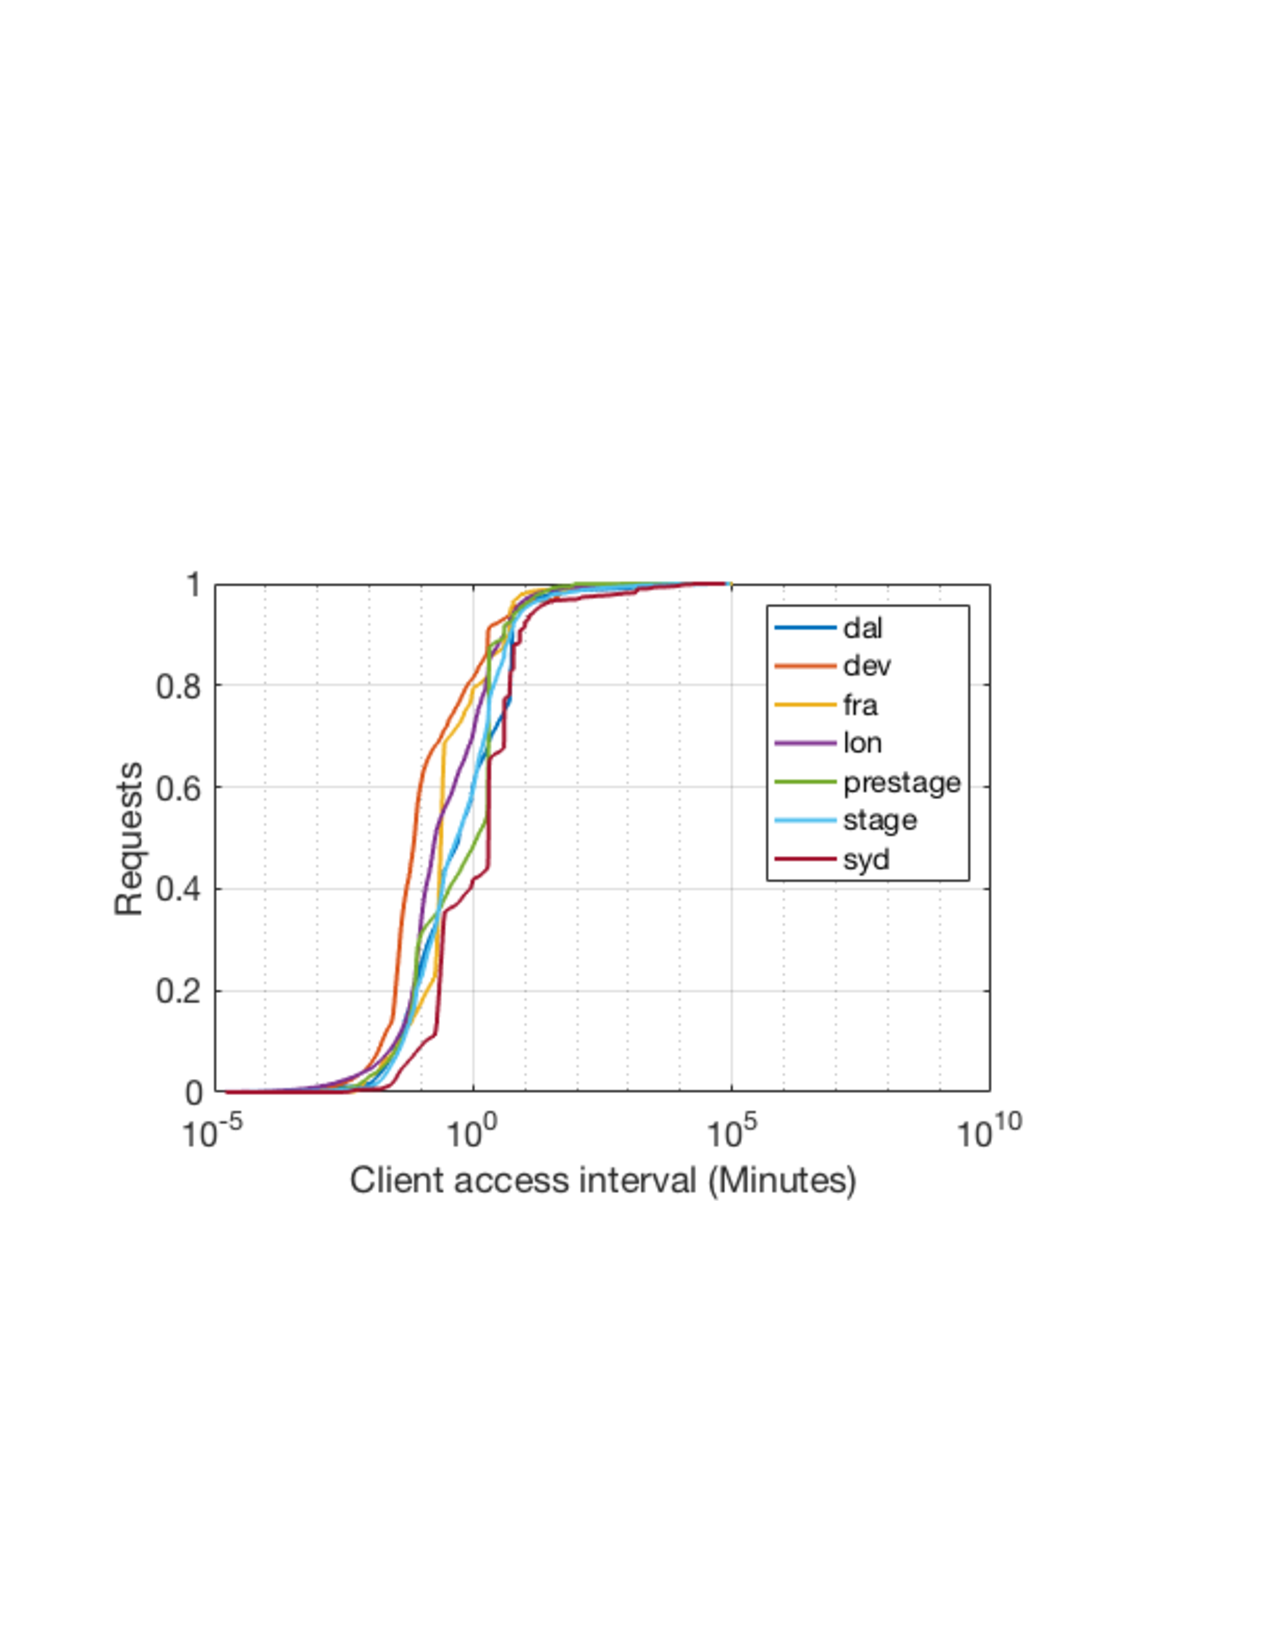
\includegraphics[width=1\textwidth]{graphs/user-intervals.pdf}
%			%\caption{PDF of client access intervals.}
%			%	\vspace{-3pt}
%			\label{fig:user-interval}
%		\end{minipage}
%	\caption{CDF of reusetime for layers, repositories and clients' access intervals.}
%	\label{fig:layer-reuse}
%\end{figure*}
\begin{figure}[t]
	\centering
	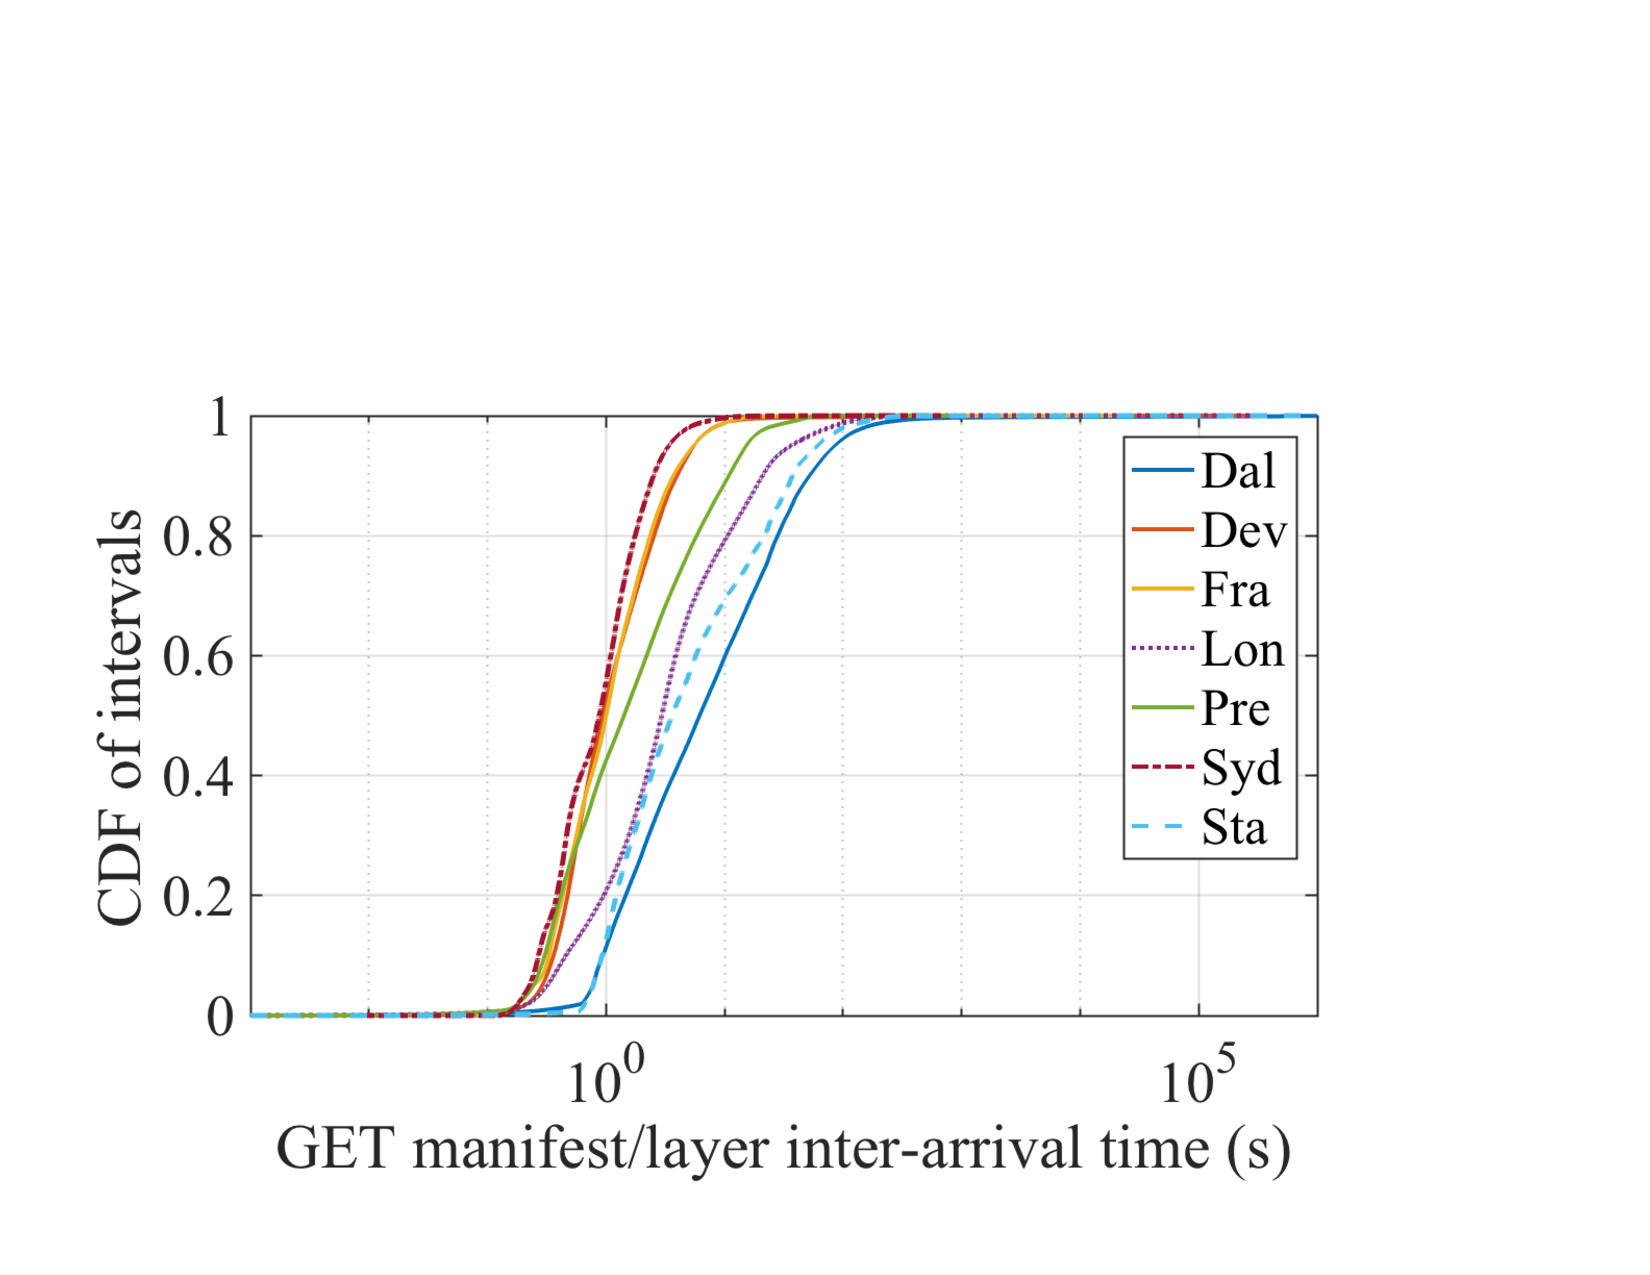
\includegraphics[width=0.3\textwidth]{graphs/GML-intervals.pdf}
	\caption{Intervals between \texttt{pull} manifest request and \texttt{pull} layer request}
	%	\vspace{-3pt}
	\label{fig:intervals}
	
\end{figure}
%\begin{figure*}[!t]
%	\centering
%	\subfigure[Layer repull count]{
%		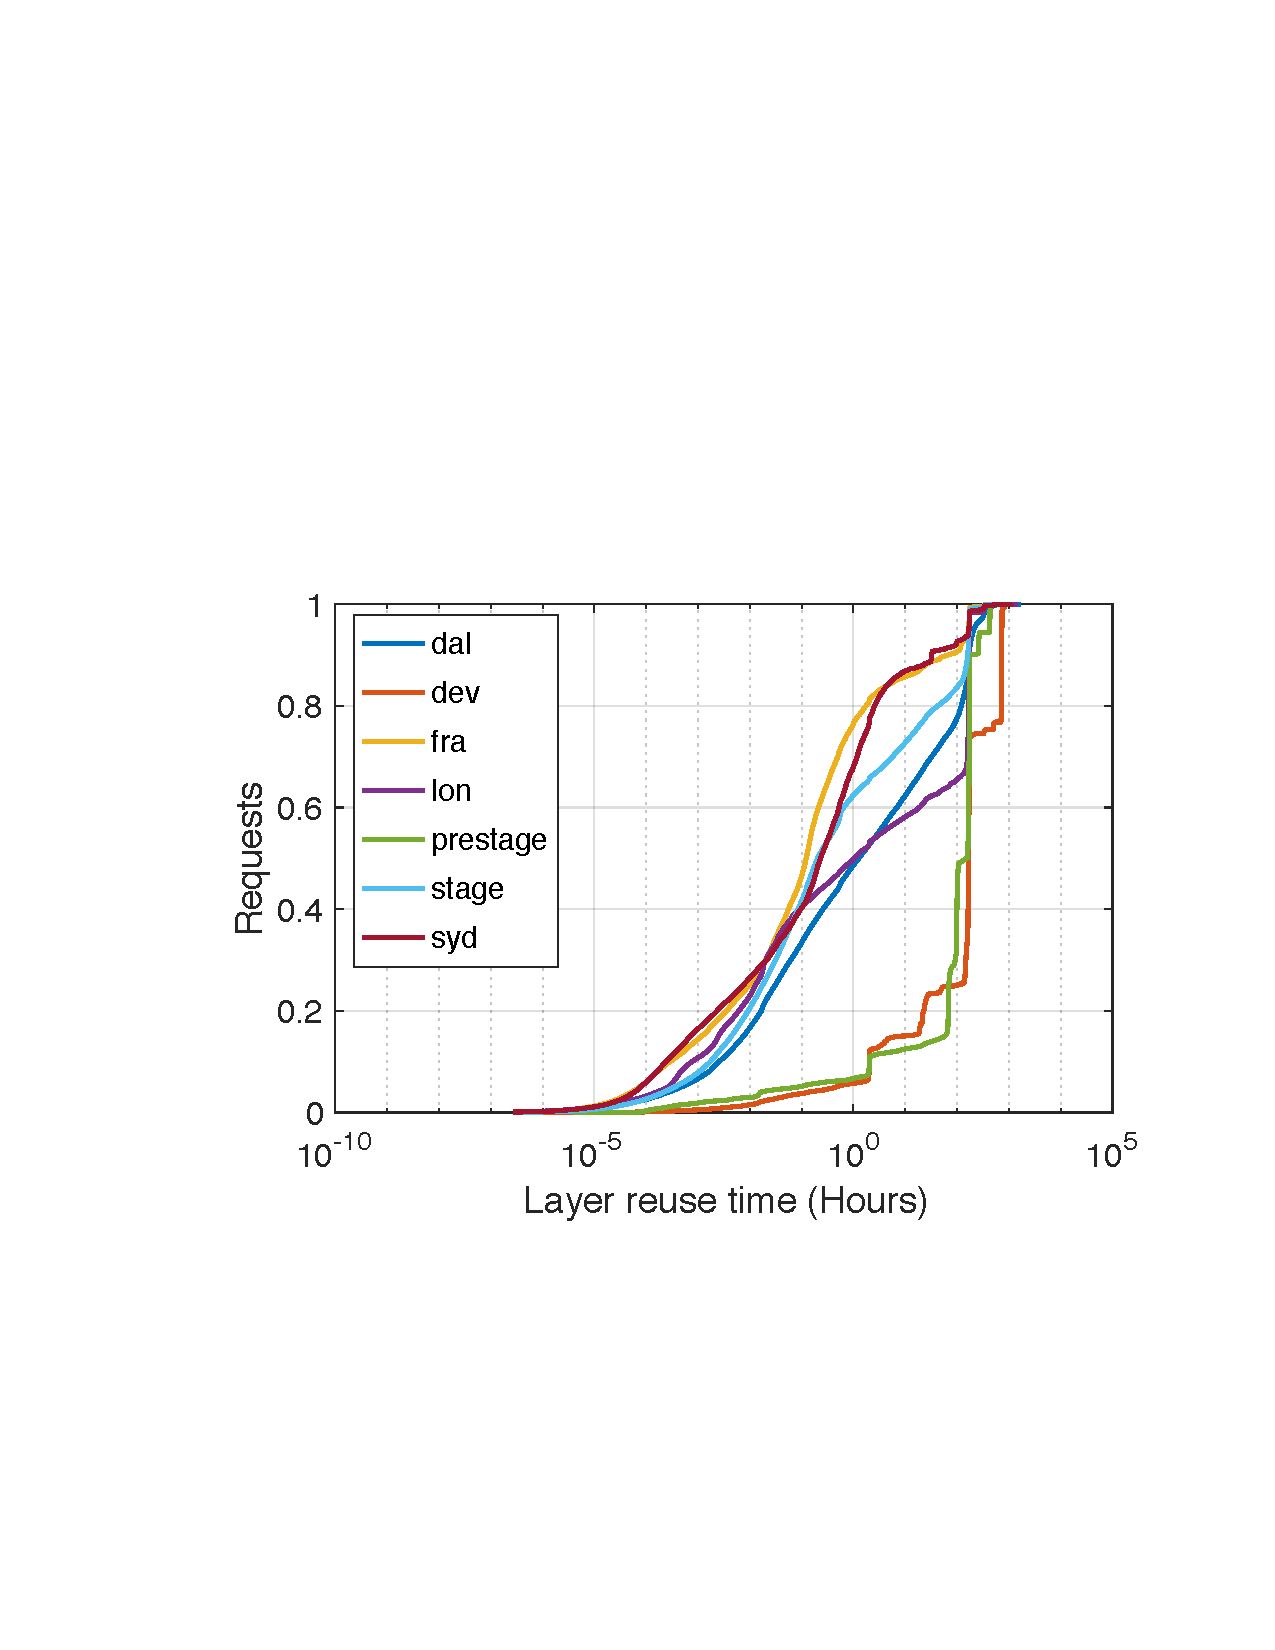
\includegraphics[width=0.2\linewidth]{graphs/layer-reusetime.pdf}
%			\label{fig:layer-reuse}
%	}
%	\subfigure[Repository repulling probability]{
%		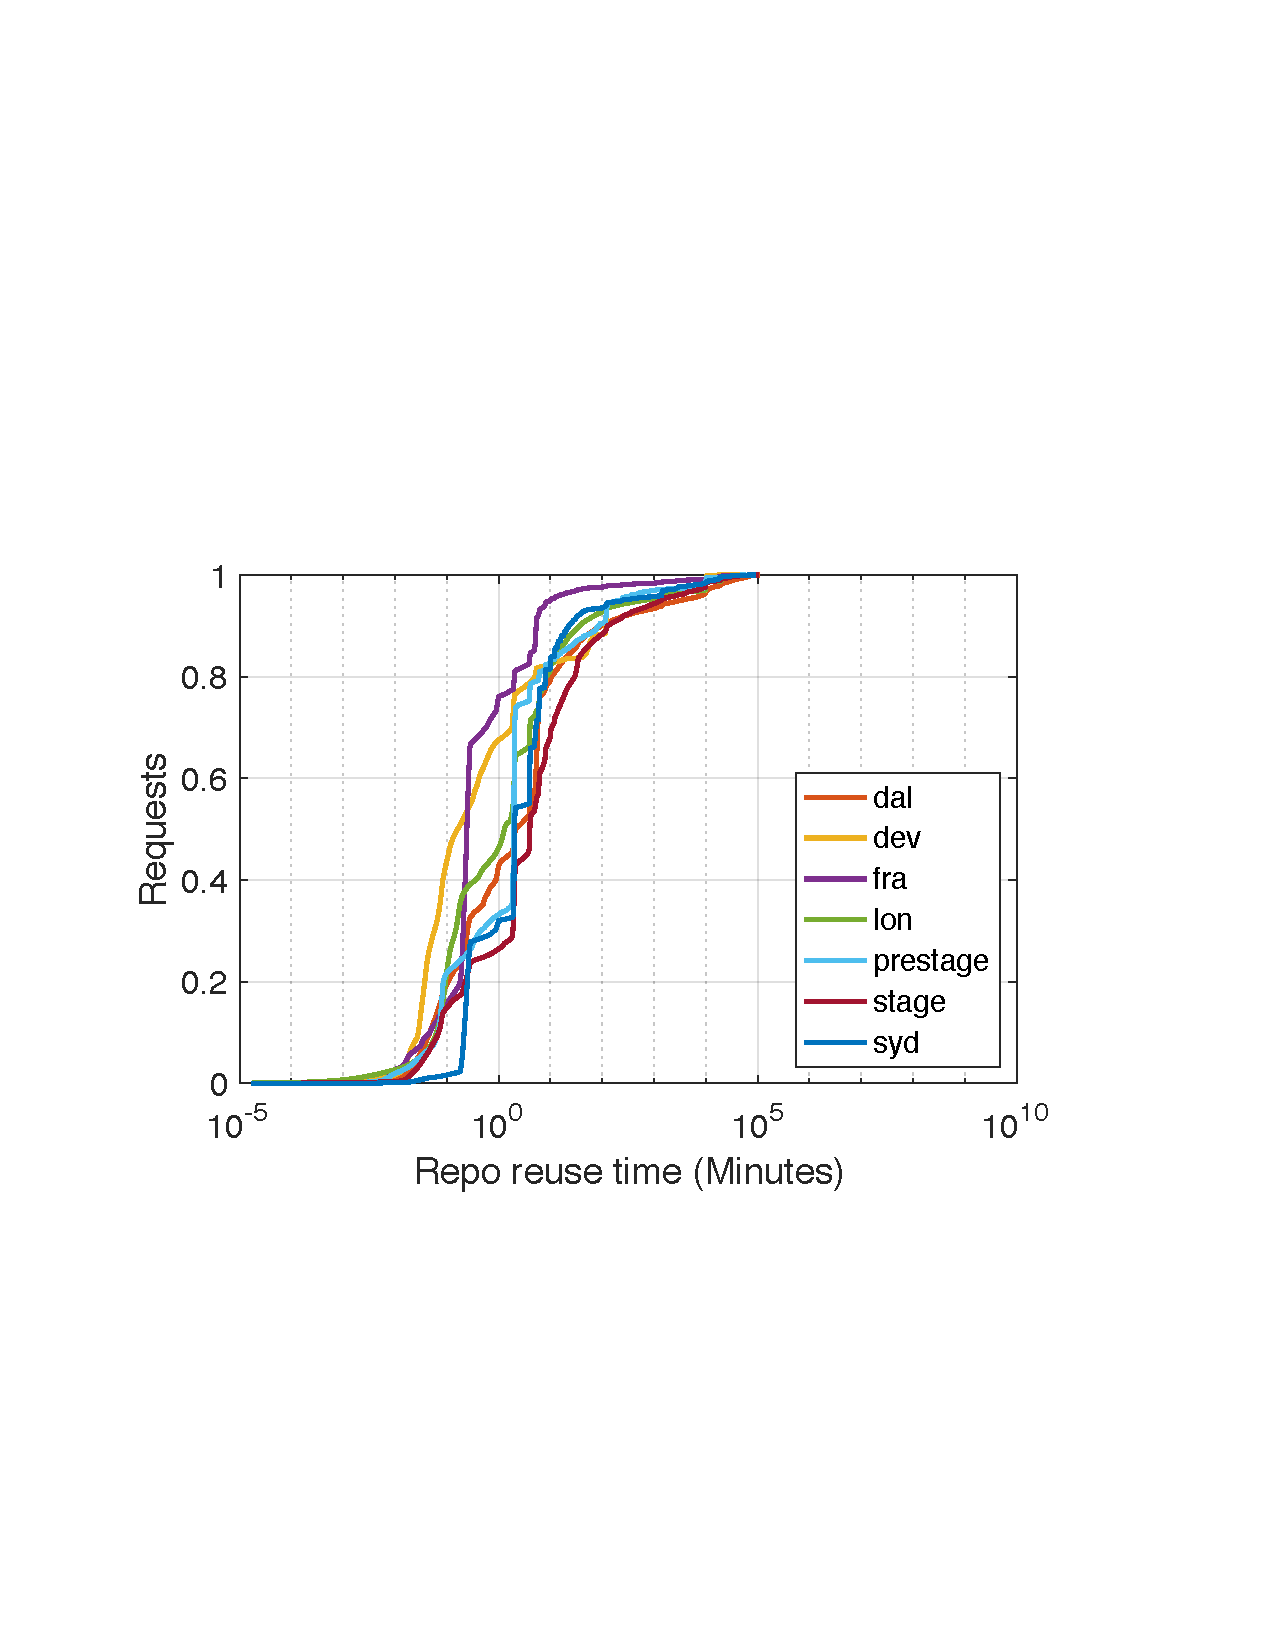
\includegraphics[width=0.2\linewidth]{graphs/repo-reusetime.pdf}
%				\label{fig:repo-reuse}
%	}
%	\subfigure[Client repulling probability]{
%		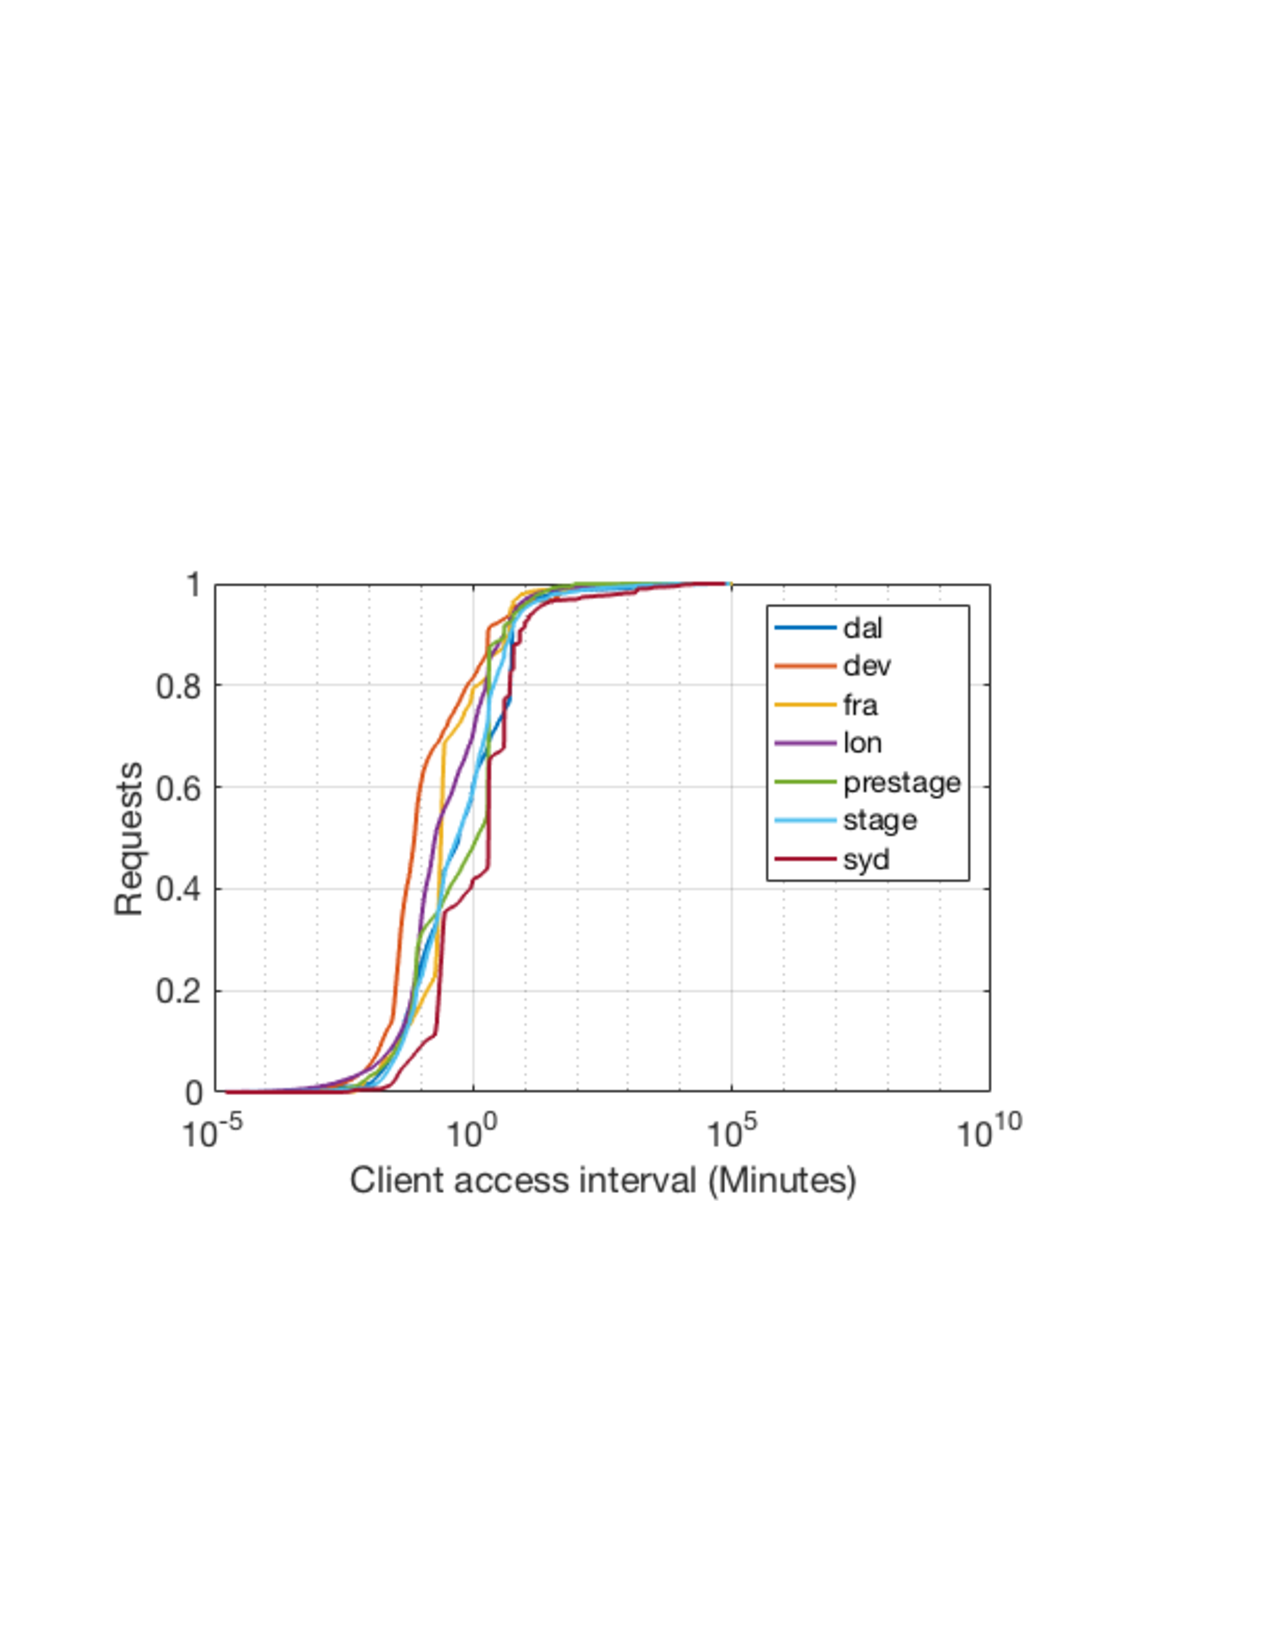
\includegraphics[width=0.2\linewidth]{graphs/user-intervals.pdf}
%			\label{fig:user-interval}
%	}
%	\caption{CDF of reusetime for layers, repositories and clients' access intervals.}
%	\label{fig:fig-reuse}
%\end{figure*}

%\begin{figure}[t]
%	\centering
%	\begin{minipage}{0.26\textwidth}
%		\centering
%		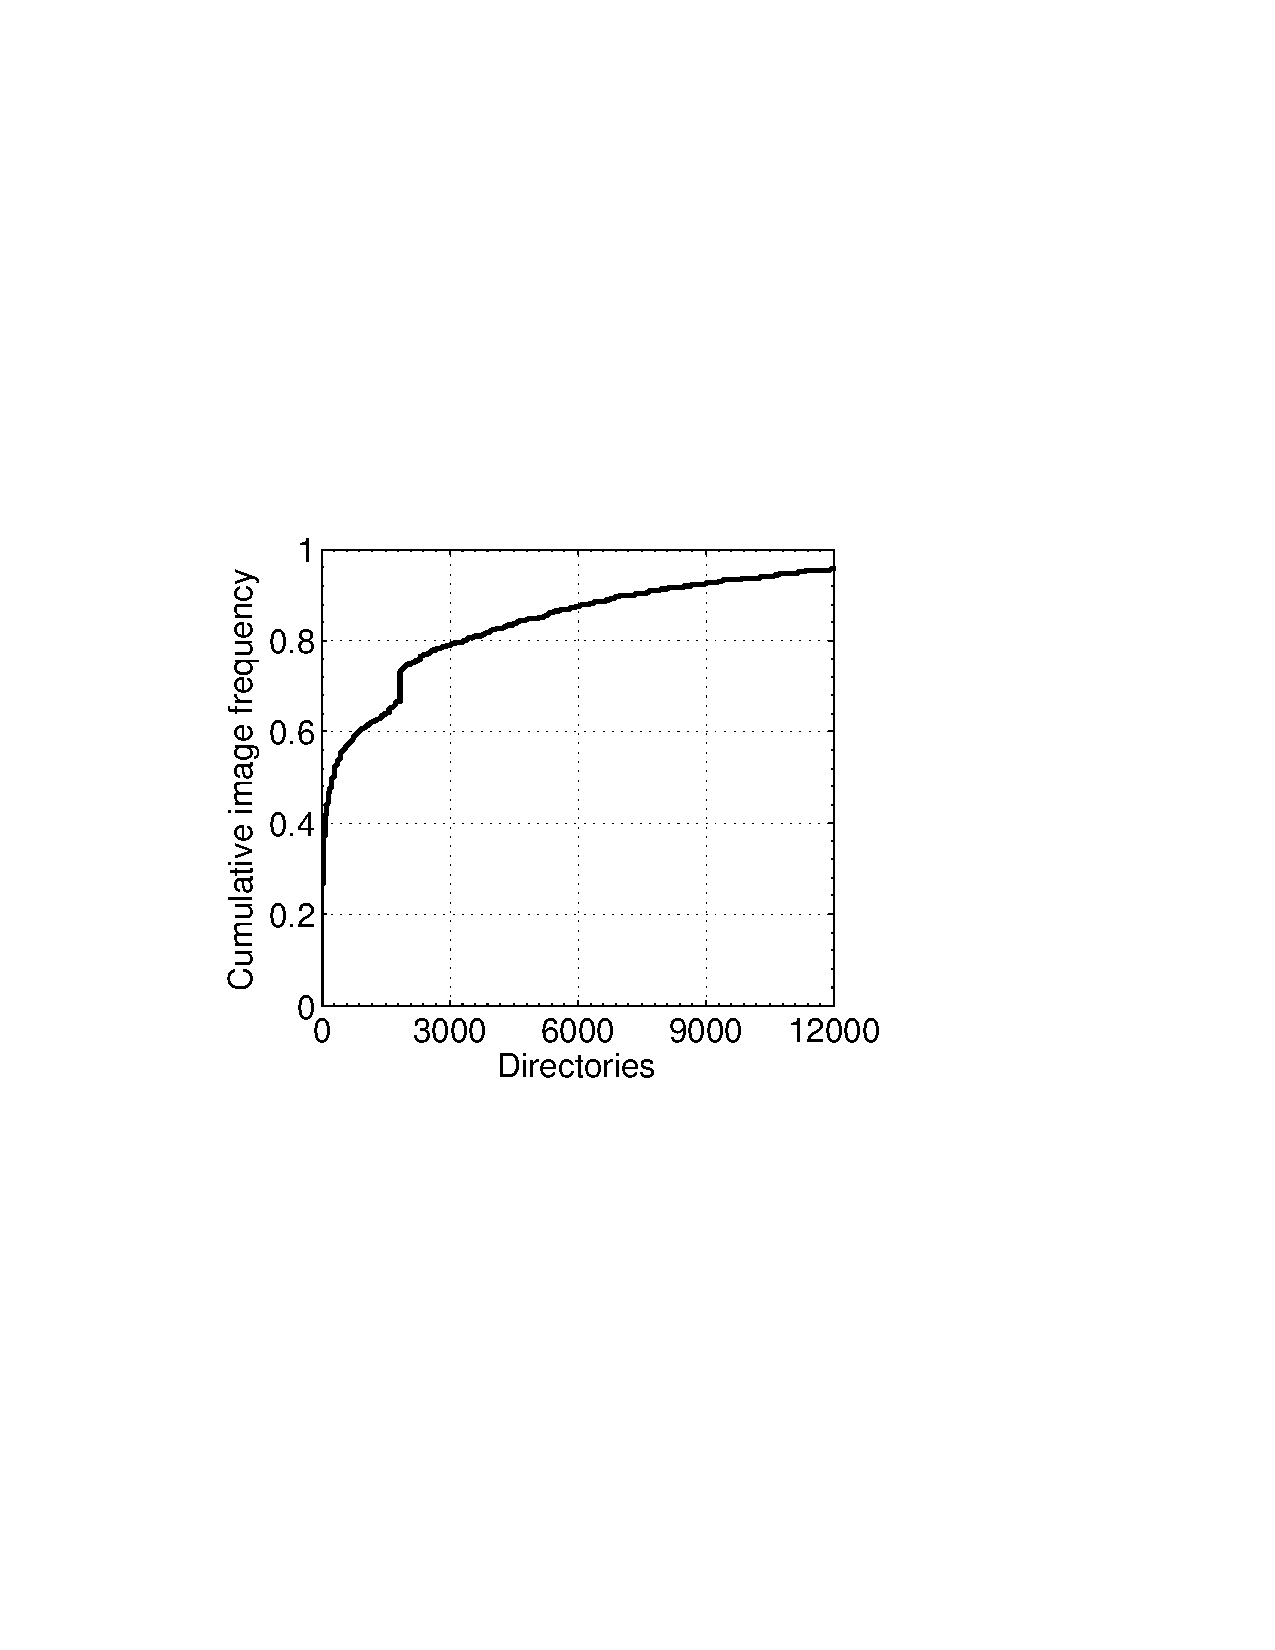
\includegraphics[width=1\textwidth]{graphs/dir.pdf}
%		\caption{CDF of images by\newline directories}
%		\label{fig-dir}
%	\end{minipage}%
%	\begin{minipage}{0.24\textwidth}
%		\centering
%		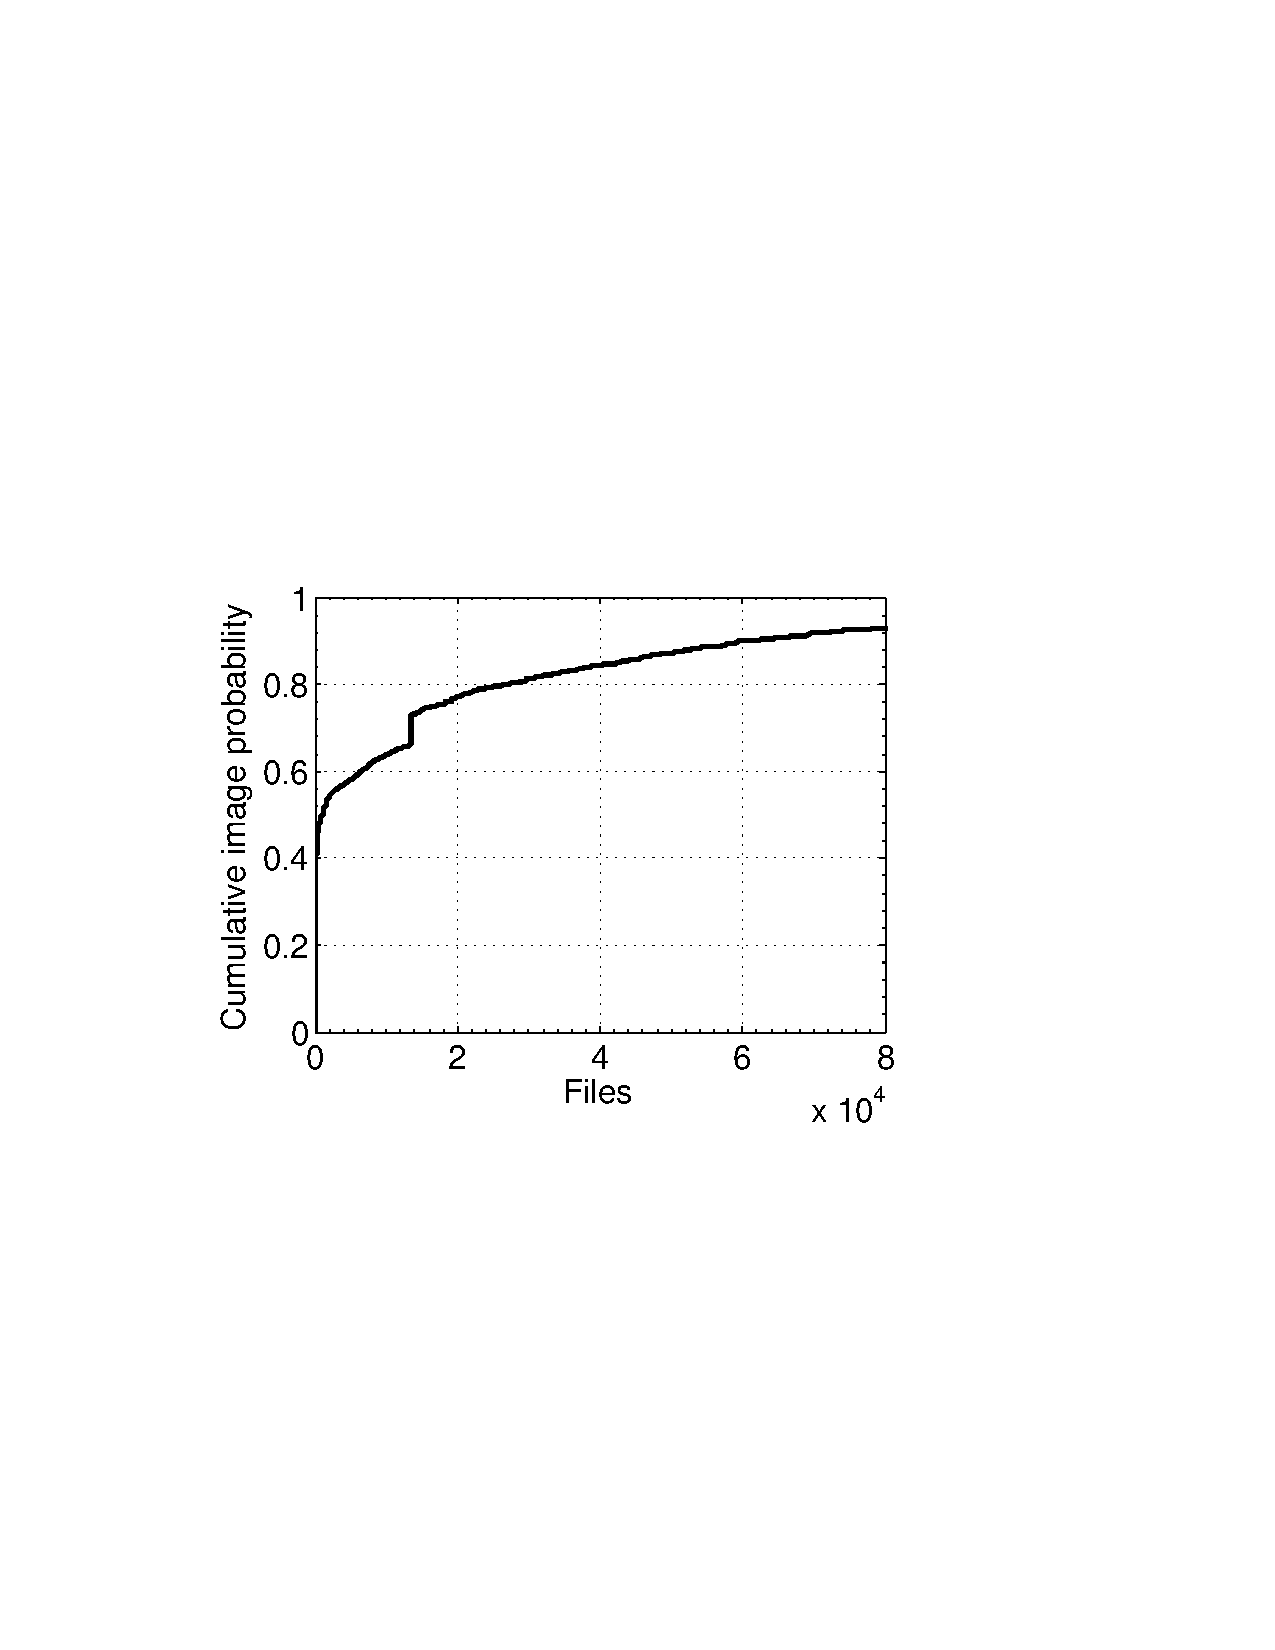
\includegraphics[width=1\textwidth]{graphs/file.pdf}
%		\caption{CDF of images by files}
%		\label{fig-file}
%	\end{minipage}
%\end{figure}

%\begin{figure}[htbp] 
%	\begin{minipage}{0.5\linewidth} 
%		\centering 
%		\includegraphics{circle} 
%		\caption{A Circle} 
%		\label{fig:circle} 
%	\end{minipage}% 
%	\begin{minipage}{0.5\linewidth} 
%		\centering 
%		\includegraphics{rectangle} 
%		\caption{A Rectangle} 
%		\label{fig:rectangle} 
%	\end{minipage} 
%\end{figure}

Figure~\ref{fig:layer-skewness} shows the CDF of layer popularity.
We observe a heavy layer access skewness for \texttt{Fra}, \texttt{Syd}, \texttt{Dal}, \texttt{Stage}, and \texttt{Lon}.
We see that 80\%, 70\%, and 60\% of the \texttt{pull} layer requests access only 10\% of layers, 
for \texttt{Fra}, \texttt{Syd}, \texttt{Dal}, \texttt{Stage}, 
and \texttt{Lon} respectively.
Figure~\ref{fig:repo-skewness} shows the CDF of repository popularity.
Compare to layer popularity, 
repository access skewness is heavier across 7 workloads.
Almost 90\% of \texttt{pull} layer requests access only 10\% of repositories for 
\texttt{Dev}, \texttt{Fra}, \texttt{Prestage}, \texttt{Syd}, and \texttt{Stage} respectively.
Almost 75\% of \texttt{pull} layer requests access only 10\% of repositories for
both \texttt{Dal} and \texttt{Lon}.
Figure~\ref{fig:client-skewness} shows the CDF of client popularity.
\texttt{Dal}, \texttt{Dev}, \texttt{Fra}, \texttt{Lon}, \texttt{Prestage}, and \texttt{Stage} shows a heavy client access skewness.
10\% of clients send 95\% \texttt{pull} layer requests for \texttt{Lon}.
\texttt{Syd} shows a slight client skewness. 70\% of requests are sent by 36\% of clients.
Overall, caching a layer with higher pull count will improve the hit ratio, 
especially for popular repositories and targeting active clients with higher repulling probability. 

Next, we analyze the layer and repository reuse time.
Layer reuse time means the duration between two consecutive requests to the same layer
while repository reuse time means the duration between two consecutive \emph{pull} manifest requests to the same repository.
Figure~\ref{fig:layer-reuse} shows the CDF of layer reuse time. 
%Layer reuse time means the duration between two consecutive \texttt{pull} requests to the same layer.
We see that layer reuse time distribution varies among different workloads.
For \texttt{Fra}, \texttt{Syd}, and \texttt{Stage},
half of the layers' reuse time is shorter than 6 minutes.
While half of layers from \texttt{Dal} and \texttt{Lon} have a reuse time higher than 1 hour.
Half of layers from both \texttt{Prestage} and \texttt{Dev} are not accessed for over 100 hours.
Consequently, for \texttt{Dal}, \texttt{Lon}, \texttt{Prestage}, and \texttt{Dev}, 
it may take longer than 1 hour for at least half newly requested layer to get a hit. 
These layers or the slices for them are unnecessarily for caching since 
their reuse time is too long and may cause other useful layers or slices to be evicted, called \emph{cache pollution}.
%Consider popular skewness, 
Figure~\ref{fig:repo-reuse} shows the CDF of repository reuse time.
%Repository reuse time means the duration between two consecutive \texttt{pull manifest} requests to the same repository.
We see that repository reuse time is much shorter than layer reuse time.
80\% of repositories are requested within 2-12 minutes across the 7 workloads.
Figure~\ref{fig:user-interval} shows the CDF of client access intervals.
client access interval means the duration between two consective requests issued by the same client.
Client access intervals are much shorter than repository reuse time.
80\% of client are active within 1 - 3 minutes for the 7 workloads. 
Hence, to eliminate \emph{cache pollution},
we consider the reuse time of layer and repository as well as client access intervals during
cache eviction.